\documentclass[UTF8,zihao=-4,fontset=windows,a4paper]{ctexart}

\usepackage{amsmath,amssymb,bm,mathtools}
\usepackage{booktabs,array,tabularx,longtable,multirow}
\usepackage{graphicx,float,caption,subcaption,placeins}
\usepackage{geometry,xcolor,hyperref,fancyhdr}
\usepackage{enumitem,xurl}
\usepackage{fvextra}
\usepackage{needspace}

\geometry{left=2.5cm,right=2.5cm,top=2.5cm,bottom=2.5cm,headheight=0pt,headsep=0pt,footskip=0.75cm}
\graphicspath{{./}}
\setmainfont{Times New Roman}
\setmonofont{Consolas}
\setCJKmainfont{SimSun}[BoldFont=SimHei]
\setCJKsansfont{SimHei}[AutoFakeBold=2]
\setCJKmonofont{FangSong}[AutoFakeBold=2]
\setlength{\parindent}{2em}
\setlength{\parskip}{0pt}
\setlength{\emergencystretch}{3em}
\linespread{1.0}\selectfont
\renewcommand{\arraystretch}{1.12}
\setlength{\tabcolsep}{5pt}
\setlist{nosep,leftmargin=2.3em}
\setcounter{secnumdepth}{0}

\ctexset{
  section={format=\centering\heiti\zihao{4},beforeskip=0.9em,afterskip=0.55em},
  subsection={format=\raggedright\heiti\zihao{-4},beforeskip=0.65em,afterskip=0.35em},
  subsubsection={format=\raggedright\songti\bfseries\zihao{-4},beforeskip=0.45em,afterskip=0.25em}
}

\captionsetup{font=small,labelsep=quad,skip=4pt}
\setlength{\floatsep}{8pt plus 2pt minus 2pt}
\setlength{\textfloatsep}{9pt plus 2pt minus 2pt}
\setlength{\intextsep}{7pt plus 1pt minus 1pt}
\renewcommand{\topfraction}{0.92}
\renewcommand{\bottomfraction}{0.82}
\renewcommand{\textfraction}{0.06}
\renewcommand{\floatpagefraction}{0.78}
\setcounter{topnumber}{3}
\setcounter{bottomnumber}{2}
\setcounter{totalnumber}{4}

\definecolor{mainblue}{RGB}{25,91,132}
\definecolor{safe}{RGB}{0,122,112}
\definecolor{danger}{RGB}{203,66,53}
\hypersetup{
  hidelinks,
  pdfauthor={},
  pdftitle={基于随机几何接触图与精确置信界的微构体导电优化},
  pdfsubject={},
  pdfkeywords={}
}
\urlstyle{same}

\pagestyle{fancy}
\fancyhf{}
\fancyfoot[C]{\thepage}
\renewcommand{\headrulewidth}{0pt}
\renewcommand{\footrulewidth}{0pt}

\newcommand{\CoverTopCell}[1]{\parbox[c][0.55cm][c]{\linewidth}{\centering\songti\zihao{5} #1}}
\newcommand{\CoverBottomCell}[1]{\parbox[c][1.34cm][c]{\linewidth}{\centering\songti\zihao{5} #1}}
\newcommand{\TemplateMatterHeading}[1]{%
  \par\addvspace{0.8em}%
  {\noindent\songti\bfseries\zihao{-4} #1\par}%
  \vspace{0.35em}%
}
\renewenvironment{abstract}{\par}{\par}
\providecommand{\tightlist}{%
  \setlength{\itemsep}{0pt}\setlength{\parskip}{0pt}}
\InputIfFileExists{build_meta.tex}{}{%
  \PackageError{paper}{Missing build_meta.tex}{Run python paper/src/build_latex.py first}}

\begin{document}
\pagenumbering{arabic}
\thispagestyle{fancy}

\noindent
\begin{tabularx}{\textwidth}{|>{\centering\arraybackslash}p{0.167\textwidth}|>{\centering\arraybackslash}X|>{\centering\arraybackslash}p{0.15\textwidth}|}
\hline
\CoverTopCell{所属类别} & \multirow{2}{=}{\centering\heiti\zihao{4}\bfseries 2026 年“华数杯”大学生数学建模竞赛} & \CoverTopCell{参赛编号} \\
\cline{1-1}\cline{3-3}
\CoverBottomCell{\PaperGroup} & & \CoverBottomCell{\PaperCompetitionId} \\
\hline
\end{tabularx}

\PaperBuildNotice

\vspace{0.45cm}
\begin{center}
  {\heiti\fontsize{15pt}{18pt}\selectfont\bfseries 基于随机几何接触图与精确置信界的微构体导电优化\par}
  \vspace{0.65cm}
  {\heiti\zihao{4}\bfseries 摘\quad{}要\par}
\end{center}

\vspace{0.25cm}
\begin{abstract}
增加导电填料能够提高介质相互接近的机会，却也会直接推高材料成本；真正决定微构体能否导通的，是随机分散的介质能否在有限空间内连成跨越两电极的完整接触链。介质形状、边界截断和随机波动都会改变这条链的形成，仅凭名义填充量或少量构型难以作出可靠设计。针对题给圆柱/球形介质填充问题，本文将截断后的每个片段视为独立凸体，以 $1.8\,\mathrm{nm}$ 间距建立三维随机几何接触图，并以 GJK 距离上下界、并查集、路径见证和精确二项置信界构成从几何判定、概率估计到成本优化的统一可复核模型。

\textbf{针对问题一，}三组附件微构体的结论依次为\textbf{不导通、导通、导通}；$144087$ 个粒子对中仅 $195$ 对进入凸体窄相判定，且与独立约束优化校验的阈值分类完全一致。

\textbf{针对问题二，}使用固定随机流的共同粒子前缀和 $20000$ 次 Monte Carlo 试验，得到 $0.50\%$、$0.60\%$、$0.70\%$ 和 $1.00\%$ 填充量下的导通概率分别为 $\mathbf{7.895\%}$、$\mathbf{22.050\%}$、$\mathbf{47.195\%}$ 和 $\mathbf{99.280\%}$，Wilson 区间与分块复算表明贯通跃迁位置稳定。

\textbf{针对问题三，}将整数填充量视为概率约束优化，对探索后冻结的候选用 $50000$ 个独立样本构造 Bonferroni--Clopper--Pearson 联合精确界。在联合 $95\%$ 置信和题定 $0.01$ 个百分点精度下，最低填充量为 $\mathbf{0.87\%}$；唯一最小粒子数尚未区分，其联合置信区间为 $\mathbf{613\le N_A^\star\le616}$。

\PaperQFourAbstract

模型可信度按三个层级检验：几何层以 $195$ 个窄相候选的 SLSQP 独立复算、距离界和逐边见证核验接触判定，阈值分类分歧为 0；随机层以互不重叠样本块、Wilson 与 Clopper--Pearson 区间对照及固定种子复现检验模拟稳定性；优化层将探索流与确认流分离，并分别对问题三的 18 个、问题四的 620 个单侧陈述控制族错误率。三层检验分别约束几何误判、抽样波动与多重筛选偏差，使关键结论均可追溯到确定的代码、随机流和机器结果。综合四问，本文在题定随机机制和截断片段独立口径下给出了从确定性导通、概率跃迁到成本选择的闭环答案；现有证据最终形成保守可行成本上界、成本证据区间和待确认边界集，并给出后续追加样本的明确对象与顺序。
\end{abstract}

\noindent\textbf{关键词：}随机几何图；连通渗流；GJK 距离；Monte Carlo 仿真；Clopper--Pearson 精确界；概率约束优化

\clearpage
\section{一、问题重述}\label{ux4e00ux95eeux9898ux91cdux8ff0}

本文研究随机分布的导电介质能否在有限微构体内部形成一条连接两侧电极的连续通路。计算域为 边长 \(10000\ \mathrm{nm}\) 的立方体，两相对的 \(x\) 向端面为带电面，其余空间由绝缘溶剂占据。 介质 A 是轴长 \(5000\ \mathrm{nm}\)、底面半径 \(30\ \mathrm{nm}\) 的直圆柱，介质 B 是半径 \(200\ \mathrm{nm}\) 的球。任意两个导电实体，或导电实体与带电面之间的集合最短距离不超过 \(1.8\ \mathrm{nm}\)，即认为二者电学接触。介质允许相交、贯穿和重叠；实体越出计算域时， 只将实际越界部分按题设边界规则映回基础立方体，并将所得截断片段分别视为独立介质。

在这一统一几何与接触定义下，需要完成以下四项任务：

\begin{enumerate}
\def\labelenumi{\arabic{enumi}.}
\tightlist
\item
  由附件给出的轴线端点重建三组有限圆柱，逐组判断左右电极是否导通，并给出可核查的贯通路径；
\item
  仅填充介质 A 时，在 \(0.50\%,0.60\%,0.70\%,1.00\%\) 四个名义体积分数下估计导通概率；
\item
  在真实导通概率不低于 \(90\%\) 的约束下，确定全 A 微构体的最低填充量；
\item
  同时填充 A、B 时，在相同概率约束下求解成本最低的整数配比。
\end{enumerate}

四问的输入形式虽分别为确定坐标、随机填充量和整数设计变量，但输出都取决于同一个二值事件： 接触网络中左右电极是否位于同一连通分量。因此，先建立可信的三维接触图，再在确定性、概率 估计和概率约束优化三个层次上调用该图模型，是全文的主线。

\section{二、问题分析}\label{ux4e8cux95eeux9898ux5206ux6790}

四个问题最终都归结为同一类连通判定：先确定导电介质之间以及介质与电极之间是否满足 \(1.8\,\mathrm{nm}\) 的距离条件，再判断这些局部接触能否形成连接左右电极的通路。计算上的主要困难在于，对所有实体对逐一进行高精度三维距离计算会带来较大的计算量，而将有限平底圆柱过度简化又可能影响临界距离附近的接触判断。

为兼顾计算效率和几何精度，本文先进行宽相（broad phase）筛选以缩小候选范围，再对剩余实体对采用 GJK 窄相（narrow phase）计算有限平底圆柱之间的距离界，并据此完成 \(1.8\,\mathrm{nm}\) 接触阈值的判定。所有确定接触边进入无向图后，再由并查集（Union-Find）判断左右电极是否连通。各问的数学对象、输出和验证重点如下。

\begin{longtable}[]{@{}lll@{}}
\caption{四个问题的数学任务与证据路线}\tabularnewline
\toprule\noalign{}
问题 & 数学任务 & 关键证据 \\
\midrule\noalign{}
\endfirsthead
\toprule\noalign{}
问题 & 数学任务 & 关键证据 \\
\midrule\noalign{}
\endhead
\bottomrule\noalign{}
\endlastfoot
一 & 确定几何与图连通 & 距离界与贯通路径 \\
二 & 伯努利期望估计 & 共同前缀、分块和概率区间 \\
三 & 一维整数概率约束 & 独立样本与联合单侧检验 \\
四 & 二维整数成本优化 & 非支配前沿与完整域穷举 \\
\end{longtable}

\textbf{针对问题一}，附件每行给出一个有限片段的轴线端点。由端点可唯一确定片段中心、方向和实际轴长，本问据此执行全对搜索（pairwise search）生成潜在接触边。有限平底圆柱的端面不同于胶囊的半球端部，端面对端时胶囊距离最多会低估两个半径。本文以胶囊距离作排除下界，再用支持映射（support mapping）和 GJK 距离界完成接触分类{[}1{]}；导通组同时给出由附件行号组成的电极间见证路径。

\textbf{针对问题二}，本文令不同介质的中心在立方体内独立均匀分布，A 的轴向服从球面各向同性 分布，并允许粒子重叠。随机杆的贯通尺度受长径比和方向分布影响{[}2{]}；有限盒的跨电极事件还 取决于边界定义。随机球模型则由球心点过程以及接触、重叠成簇规则共同确定{[}3{]}。本文据此直接 生成有限盒内的随机几何图，把每个微构体是否导通记为伯努利变量。借鉴 Newman--Ziff 逐个激活 节点并增量维护连通簇的思想{[}4{]}，同一试验只生成一次最大粒子前缀，记录首次导通粒子数，即可 同时回答四个填充量，并从算法结构上保证概率随粒子数不下降。

\textbf{针对问题三}，决策变量是整数 \(N_A\)，约束为未知真实概率 \(p_A(N_A)\ge0.90\)。本文对 临界整数采用统一的 \(100000\) 次样本，Wilson 区间描述比例波动{[}5{]}，Clopper--Pearson 单侧精确限{[}6{]}与 Bonferroni 联合校正{[}7{]}完成门槛分类，固定样本量保证区间覆盖含义{[}8{]}。

\textbf{针对问题四}，按``同时填充''将决策变量限定为正整数对 \((N_A,N_B)\)。每条左右路径所需的最大 A 序号和最大 B 序号形成二维激活标签；保留非支配前沿后，一张最大静态图能够同时回答多个配比。预先确定的低成本候选域包含 37 个正整数混合配比，并加入 4 个全 A 参照；统一计算 41 个设计的联合单侧精确下限后，在混合候选域内按可行性与精确成本排序。

图 \ref{fig:model-workflow} 汇总四问共用的计算对象、程序顺序与校验关系：几何实体先经统一距离核 生成接触图，问题一读取确定性连通，问题二至四依次叠加概率估计、一维临界判断和二维成本约束。

\begin{figure}[htbp]
  \centering
  
\includegraphics[width=0.96\textwidth]{figures/model_workflow.png}
  \caption{微构体导电优化的五模块计算与证据流程。A，几何合同与随机微结构；B，统一接触图引擎；C，边界、单调性与独立确认原则；D，概率估计和临界阈值确认；E，成本前沿与置信可行方案。}
  \label{fig:model-workflow}
\end{figure}

\section{三、模型假设与符号说明}\label{ux4e09ux6a21ux578bux5047ux8bbeux4e0eux7b26ux53f7ux8bf4ux660e}

\subsection{3.1 模型假设}\label{ux6a21ux578bux5047ux8bbe}

\begin{enumerate}
\def\labelenumi{\arabic{enumi}.}
\tightlist
\item
  以立方体中心为坐标原点，左右电极分别为 \(x=-L/2\) 与 \(x=L/2\) 两个端面；绝缘溶剂不 形成图节点，其他四个盒面不作为电极。
\item
  不同介质相互独立。实体越界后，仅将实际越界部分映回基础立方体；每个截断片段均作为 独立介质节点，不因来自同一原实体而额外增加内部连接边。
\item
  问题二至四中，各介质中心独立服从 \(\Omega\) 上的均匀分布。介质 A 的方位角均匀， \(\cos\theta\) 在 \([-1,1]\) 上均匀，即其轴向在单位球面上各向同性。
\item
  介质允许相交、贯穿和重叠，不进行硬核排斥采样；体积分数按所有原始粒子的名义体积之和 计算，不扣除重叠体积，也不因边界截断重新计量。
\item
  本文以距离阈值接触图中的左右贯通作为导通判据，输出贯通状态与导通概率。若给定电阻率、 接触电阻、电压和隧穿衰减参数，可在同一接触图上进一步求解等效电阻与电流分布。
\item
  两实体间距离等于 \(1.8\ \mathrm{nm}\) 时归入接触；数值计算由距离上下界完成分类，区间跨越 阈值时继续收紧精度，直至上下界落在阈值同一侧。
\item
  A 的随机仿真按圆柱中心线与盒面交点切段，并将各段表示为有限平底圆柱。该边界算子在四问中保持一致，可直接进入平底圆柱支持映射、GJK 距离判定和接触图构建。
\end{enumerate}

\subsection{3.2 主要符号}\label{ux4e3bux8981ux7b26ux53f7}

\begin{longtable}[]{@{}
  >{\raggedright\arraybackslash}p{(\linewidth - 4\tabcolsep) * \real{0.3400}}
  >{\raggedright\arraybackslash}p{(\linewidth - 4\tabcolsep) * \real{0.5400}}
  >{\centering\arraybackslash}p{(\linewidth - 4\tabcolsep) * \real{0.1200}}@{}}
\caption{主要符号及定义}\tabularnewline
\toprule\noalign{}
\begin{minipage}[b]{\linewidth}\raggedright
符号
\end{minipage} & \begin{minipage}[b]{\linewidth}\raggedright
含义
\end{minipage} & \begin{minipage}[b]{\linewidth}\centering
单位
\end{minipage} \\
\midrule\noalign{}
\endfirsthead
\toprule\noalign{}
\begin{minipage}[b]{\linewidth}\raggedright
符号
\end{minipage} & \begin{minipage}[b]{\linewidth}\raggedright
含义
\end{minipage} & \begin{minipage}[b]{\linewidth}\centering
单位
\end{minipage} \\
\midrule\noalign{}
\endhead
\bottomrule\noalign{}
\endlastfoot
\(\Omega=[-L/2,L/2]^3\) & 微构体计算域，\(L=10000\) & \(\mathrm{nm}\) \\
\(E_L,E_R\) & 左右带电面 \(x=\mp L/2\) & - \\
\(p_i^-,p_i^+,c_i,u_i,\ell_i\) & 第 \(i\) 个圆柱的轴端点、中心、单位方向和轴长 & \(\mathrm{nm}\) \\
\(C_i\) & 由第 \(i\) 个片段形成的有限平底圆柱集合 & - \\
\(r_A,\ell_A\) & A 的半径与轴长，分别为 \(30,5000\) & \(\mathrm{nm}\) \\
\(r_B\) & B 的半径，\(r_B=200\) & \(\mathrm{nm}\) \\
\(\delta\) & 接触阈值，\(\delta=1.8\) & \(\mathrm{nm}\) \\
\(N_A,N_B\) & 两类介质的粒子数 & 个 \\
\(d_{ij}\) & 两个有限实体的集合最短距离 & \(\mathrm{nm}\) \\
\(G=(V,E)\) & 介质片段与电极构成的无向接触图 & - \\
\(Y_s\) & 第 \(s\) 个微构体的导通指标 & - \\
\(p,\widehat p\) & 真实导通概率与蒙特卡洛（Monte Carlo）估计 & - \\
\(T_s\) & 第 \(s\) 个全 A 序列的首次导通粒子数 & 个 \\
\(n,k_N\) & 固定试验数与前缀 \(N\) 下的导通次数 & 次 \\
\(z_{0.975}\) & 标准正态分布的 \(97.5\%\) 分位数 & - \\
\(C,W\) & 总成本与精确整数成本权重 & 元 \\
\end{longtable}

\section{四、随机几何接触图模型}\label{ux56dbux968fux673aux51e0ux4f55ux63a5ux89e6ux56feux6a21ux578b}

\subsection{4.1 有限圆柱与电极距离}\label{ux6709ux9650ux5706ux67f1ux4e0eux7535ux6781ux8dddux79bb}

附件第 \(i\) 行给出圆柱片段的轴线端点 \(p_i^-\) 和 \(p_i^+\)。由此可确定其实际轴长、中心和单位方向：

\[
\ell_i=\lVert p_i^+-p_i^-\rVert,
\qquad
c_i=\frac{p_i^-+p_i^+}{2},
\qquad
u_i=\frac{p_i^+-p_i^-}{\ell_i}.
\]

相应的有限平底圆柱表示为

\[
C_i=\left\{c_i+t u_i+v:
|t|\leq\frac{\ell_i}{2},\quad
v\cdot u_i=0,\quad
\lVert v\rVert\leq r_A\right\}.
\]

该集合保留了与 \(u_i\) 垂直的两个圆形端面，与半球封端的胶囊体具有不同的端部几何。为直接计算凸体距离，本文采用支持映射。令

\[
q_{\perp}=q-(q\cdot u_i)u_i,
\]

则有限圆柱沿方向 \(q\) 的支持点为

\[
s_{C_i}(q)=c_i
+\frac{\ell_i}{2}\operatorname{sgn}(q\cdot u_i)u_i
+r_A\frac{q_{\perp}}{\lVert q_{\perp}\rVert}.
\]

当 \(q_{\perp}=0\) 时，径向项取零。两个凸体的最短距离等于 Minkowski 差集 \(C_i-C_j\) 到原点的距离。GJK（Gilbert--Johnson--Keerthi）算法通过两个实体的支持映射，在至多四个点构成的单纯形上迭代求解该距离{[}1{]}，无需将圆柱曲面离散为三角网格。设当前单纯形中距原点最近的点为 \(p\)，沿 \(-p\) 方向取得的新支持点为 \(s\)，则距离上下界为

\[
L=\max\left\{0,\frac{p\cdot s}{\lVert p\rVert}\right\}
\leq d(C_i,C_j)\leq
\lVert p\rVert=U.
\]

当 \(U\leq\delta\) 时判定接触；当 \(L>\delta\) 时判定分离；若 \(L\leq\delta<U\)，则继续迭代并收紧计算容差。

GJK 仅用于少量候选对的窄相判定。进入窄相前，先由轴对齐包围盒或空间网格生成邻近候选，再对候选轴段计算胶囊间隙：

\[
d_{ij}^{\mathrm{cap}}
=\max\left\{0,
d\!\left([p_i^-,p_i^+],[p_j^-,p_j^+]\right)-2r_A
\right\}.
\]

有限平底圆柱包含于相应胶囊体，因此

\[
d_{ij}^{\mathrm{cap}}\leq d(C_i,C_j).
\]

当 \(d_{ij}^{\mathrm{cap}}>\delta\) 时，该实体对可在宽相中排除；其余候选进入有限圆柱 GJK 判定。宽相仅承担候选排除，最终接触分类仍以有限平底圆柱的距离界为准。

圆柱在 \(x\) 方向上的投影半宽为

\[
a_i=\frac{\ell_i}{2}|u_{ix}|+r_A\sqrt{1-u_{ix}^{2}},
\]

故其 \(x\) 投影区间为 \([c_{ix}-a_i,\,c_{ix}+a_i]\)。设电极所在平面为 \(x=x_e\)，圆柱到电极的间隙为

\[
d(C_i,E_e)=\max\left\{0,|c_{ix}-x_e|-a_i\right\}.
\]

边界片段均位于基础立方体内，因此电极接触边可由上述投影公式闭式判定，无需调用 GJK。

\subsection{4.2 边界片段与接触图}\label{ux8fb9ux754cux7247ux6bb5ux4e0eux63a5ux89e6ux56fe}

在本文采用的 A 类介质边界算子中，越界圆柱按中心线与盒面的交点切分。盒内部分保持原位，实际越界部分沿对应坐标方向平移一个盒长后映回基础域 \(\Omega\)。若圆柱同时跨越多个坐标面，则分别沿各坐标方向完成切分与映回。

映回后的每个片段均作为独立图节点，同源片段之间不自动添加内部连接边。片段间距离采用基础域内的直接欧氏距离；对于未发生实际越界的独立介质，不使用最小镜像（minimum-image）规则补充周期接触边。介质 B 的越界球片在问题四中按球与胞盒的凸交集处理。

设介质片段节点集合为 \(V_M\)，则无向接触图定义为

\[
G=(V,E),\qquad V=V_M\cup\{E_L,E_R\},
\]

\[
E=\left\{(i,j):d_{ij}\leq\delta\right\}
\cup
\left\{(i,E_e):d(C_i,E_e)\leq\delta\right\},
\qquad E_e\in\{E_L,E_R\}.
\]

微构体导通当且仅当左右电极位于同一连通分量，即

\[
\operatorname{find}(E_L)=\operatorname{find}(E_R).
\]

Union-Find 用于增量维护接触图的连通分量。每个节点初始自成集合，发现接触边后合并其两端节点；路径压缩与按集合大小合并使单次操作具有近常数的均摊开销。Union-Find 给出电极是否贯通；若需要恢复具体路径，则在同一确定边集上执行 BFS，并由前驱节点反向得到 \(E_L\) 到 \(E_R\) 的最短边数路径。

\begin{longtable}[]{@{}rl@{}}
\caption{确定性接触图的判定伪代码}\tabularnewline
\toprule\noalign{}
步骤 & 确定性接触图判定伪代码 \\
\midrule\noalign{}
\endfirsthead
\toprule\noalign{}
步骤 & 确定性接触图判定伪代码 \\
\midrule\noalign{}
\endhead
\bottomrule\noalign{}
\endlastfoot
输入 & 有限实体集合、左右电极与接触阈值 \(\delta\) \\
1 & 计算各实体的包围盒、胶囊距离下界与电极投影，建立电极接触边 \\
2 & 生成 broad phase 候选；若距离下界大于 \(\delta\)，排除该实体对 \\
3 & 对剩余候选调用 GJK；仅在距离上界不超过 \(\delta\) 时加入接触边 \\
4 & 每加入一条确定接触边，即在 Union-Find 中合并两端节点 \\
5 & 比较 \(E_L\) 与 \(E_R\) 的根节点；若相同，则使用 BFS 恢复见证路径 \\
输出 & 导通状态、确定接触边及可选的电极间见证路径 \\
\end{longtable}

对于 \(M\) 个片段，朴素全对搜索的最坏复杂度为 \(O(M^2)\)。若宽相将候选压缩至 \(K\) 对，且单对 GJK 的最大迭代次数为 \(I\)，则窄相的计算量为 \(O(KI)\)。Union-Find 处理节点和接触边的均摊复杂度为 \(O((M+\lvert E\rvert)\alpha(M))\)，其中 \(\alpha\) 为反 Ackermann 函数；BFS 的复杂度为 \(O(M+\lvert E\rvert)\)。随机大样本中进一步采用空间哈希（spatial hashing）限制候选邻域，从而减小实际进入 GJK 的候选规模 \(K\)，最坏复杂度阶数仍为 \(O(M^2)\)。

\subsection{4.3 随机生成与共同前缀}\label{ux968fux673aux751fux6210ux4e0eux5171ux540cux524dux7f00}

对第 \(s\) 次试验，介质中心独立生成于 \(c_i\sim U(\Omega)\)。介质 A 的轴向服从球面各向同性分布，具体取

\[
\varphi\sim U[0,2\pi),\qquad \mu=\cos\theta\sim U[-1,1],
\]

并令

\[
u=\left(\sqrt{1-\mu^2}\cos\varphi,
\sqrt{1-\mu^2}\sin\varphi,\mu\right).
\]

均匀抽取 \(\theta\) 会造成单位球面上的取向偏置；均匀抽取 \(\mu=\cos\theta\) 才能得到恒定的球面面积概率密度。所有随机量由固定根种子与试验序号确定，使同一配置能够重复生成完全一致的输入序列。

对同一次试验，先生成长度为 \(N_{\max}\) 的有序粒子序列，再以其前 \(N\) 个原始粒子构成规模为 \(N\) 的微构体。新增粒子只会增加片段、接触边和电极边，不会删除已有图结构，因此导通事件关于 \(N\) 单调不减。定义第 \(s\) 次试验在粒子数 \(N\) 下的导通指标和首次导通粒子数为

\[
Y_s(N)=\mathbf 1\{E_L\leftrightarrow E_R\text{ in }G_s(N)\},\qquad
T_s=\inf\{N:Y_s(N)=1\}.
\]

则 \(Y_s(N)=\mathbf 1\{T_s\leq N\}\)。同一次试验中的多个填充量共用同一条有序粒子前缀，因此既可复用几何计算，又具有样本级单调性：

\[
Y_s(354)\leq Y_s(424)\leq Y_s(495)\leq Y_s(707).
\]

固定 \(n\) 个独立试验后，粒子数 \(N\) 下的导通次数及概率估计为

\[
k_N=\sum_{s=1}^n\mathbf 1\{T_s\leq N\},\qquad
\widehat p_A(N)=\frac{k_N}{n}.
\]

共同前缀模拟的执行顺序、停止规则与统一统计关系见表 \ref{tab:q2-shared-prefix-pseudocode}。

\begin{table}[H]
\centering
\caption{共同随机前缀 Monte Carlo 伪代码}
\label{tab:q2-shared-prefix-pseudocode}
\begin{tabular}{@{}rl@{}}
\toprule
步骤 & 全 A 共同前缀模拟伪代码 \\
\midrule
输入 & 最大粒子数 \(N_{\max}\)、固定试验数 \(n\) 与根种子 \\
1 & 生成 \(N_{\max}\) 个独立中心和各向同性方向 \\
2 & 按序激活粒子片段，并查询 spatial hashing 中的已激活邻近候选 \\
3 & 依次执行 broad phase、GJK narrow phase 与 Union-Find 合并 \\
4 & 两电极首次位于同一连通分量时记录 \(T_s\)，结束本次试验 \\
5 & 至 \(N_{\max}\) 仍未贯通时记录 \(T_s=N_{\max}+1\) \\
6 & 按查询前缀 \(N\) 统计 \(T_s\leq N\)，计算成功数、概率与区间 \\
输出 & 各试验的 \(T_s\)，以及各查询前缀的成功数、概率估计和置信区间 \\
\bottomrule
\end{tabular}
\end{table}

一次 \(N_{\max}\) 前缀即可同时回答四个填充量，避免分别生成四套随机几何图。设第 \(s\) 次试验在记录 \(T_s\) 前共检索 \(K_s\) 个空间候选，GJK 的累计迭代次数为 \(J_s\)，则其主要计算量为 \(O(K_s+J_s)\)。Union-Find 随粒子激活增量更新，存储量主要由当前片段、空间哈希桶、确定接触边和连通分量决定。

\subsection{4.4 伯努利（Bernoulli）概率与 Wilson 区间}\label{ux4f2fux52aaux5229ux6982ux7387ux4e0e-wilson-ux533aux95f4}

对于固定粒子数 \(N\)，各独立试验的导通指标 \(Y_s(N)\) 服从参数为 \(p_A(N)\) 的 Bernoulli 分布，因此 \(k_N\sim\operatorname{Bin}(n,p_A(N))\)。点估计 \(\widehat p=k_N/n\) 给出样本导通比例。问题二采用双侧 \(95\%\) Wilson 得分区间{[}5{]}描述有限样本不确定性。令 \(z=z_{0.975}\)，区间中心与半宽为

\[
c_W=\frac{\widehat p+z^2/(2n)}{1+z^2/n},\qquad
h_W=\frac{z}{1+z^2/n}
\sqrt{\frac{\widehat p(1-\widehat p)}{n}+\frac{z^2}{4n^2}},
\]

于是 \([p_L,p_U]=[c_W-h_W,c_W+h_W]\)。Wilson 区间通过得分方程同时调整区间中心与宽度，在概率接近 0 或 1 时仍具有较好的端点表现。本文所有区间均在预先固定的样本量 \(n\) 上计算。同一次试验中的不同前缀共享粒子序列，因此不同 \(N\) 下的导通指标存在相关性；对于任一固定 \(N\)，不同试验仍相互独立，故可分别给出其边际 Wilson 区间。问题二使用双侧 Wilson 区间描述概率曲线，问题三和问题四则使用 Bonferroni 校正的单侧 Clopper--Pearson 精确限{[}6{]}完成概率约束判定。

\section{五、各问题的求解}\label{ux4e94ux5404ux95eeux9898ux7684ux6c42ux89e3}

\subsection{5.1 问题一：附件微构体的确定性判定}\label{ux95eeux9898ux4e00ux9644ux4ef6ux5faeux6784ux4f53ux7684ux786eux5b9aux6027ux5224ux5b9a}

\subsubsection{5.1.1 实体重建与求解流程}\label{ux5b9eux4f53ux91cdux5efaux4e0eux6c42ux89e3ux6d41ux7a0b}

附件每条有效记录含六个坐标，先按第 4.1 节公式重建一根实际轴长为 \(\ell_i\) 的平底圆柱，并以原工作表行号记为 \(r_i\)。三组分别得到 \(12,49,535\) 个独立片段。计算依次执行：坐标与轴长检查；圆柱到左右电极的闭式投影；全部行对的胶囊宽相；候选对的平底圆柱 GJK 窄相；确定边集上的 Union-Find 判定；以及导通组的 BFS 见证恢复。每个片段均按附件端点给出的实际轴长重建。

在最大的一组中，全对搜索仍只有 \(\binom{535}{2}=142845\) 对，确定性穷举（exhaustive search）可以直接得到全部接触关系。三组宽相与窄相统计如下。

\begingroup
\setlength{\tabcolsep}{3pt}
\begin{table}[H]
\centering
\caption{问题一的宽相筛选与窄相判定统计}
\begin{tabular}{@{}
  >{\raggedright\arraybackslash}p{(\linewidth - 14\tabcolsep) * \real{0.0900}}
  >{\centering\arraybackslash}p{(\linewidth - 14\tabcolsep) * \real{0.1200}}
  >{\centering\arraybackslash}p{(\linewidth - 14\tabcolsep) * \real{0.1250}}
  >{\centering\arraybackslash}p{(\linewidth - 14\tabcolsep) * \real{0.1250}}
  >{\centering\arraybackslash}p{(\linewidth - 14\tabcolsep) * \real{0.1250}}
  >{\centering\arraybackslash}p{(\linewidth - 14\tabcolsep) * \real{0.1250}}
  >{\centering\arraybackslash}p{(\linewidth - 14\tabcolsep) * \real{0.1250}}
  >{\centering\arraybackslash}p{(\linewidth - 14\tabcolsep) * \real{0.1650}}@{}}
\toprule
分组 & 片段数 & 全部行对 & broad phase & narrow phase & 确定接触 & 确定分离 & 电极接触边 \\
\midrule
组 1 & 12 & 66 & 64 & 2 & 2 & 0 & 7 \\
组 2 & 49 & 1176 & 1149 & 27 & 27 & 0 & 22 \\
组 3 & 535 & 142845 & 142679 & 166 & 165 & 1 & 182 \\
\bottomrule
\end{tabular}
\end{table}
\endgroup

三组共枚举 \(144087\) 个粒子对，其中 \(143892\) 对由宽相排除，\(195\) 对进入 GJK；胶囊下界将高精度计算集中到总行对的 \(0.1353\%\)。唯一经窄相判为分离的候选位于组 3，其距离下界为 \(11.9342105384\ \mathrm{nm}\)；其余 \(194\) 个候选均为确定接触。

\subsubsection{5.1.2 导通结论与路径见证}\label{ux5bfcux901aux7ed3ux8bbaux4e0eux8defux5f84ux89c1ux8bc1}

把全部确定接触边与电极边写入同一个无向图后，组 1 的左右电极属于不同连通分量，组 2、 组 3 的左右电极属于同一连通分量。结果及 BFS 恢复的最短边数见证为

\begin{longtable}[]{@{}ccc@{}}
\caption{附件三组微构体的确定性导通判定}\tabularnewline
\toprule\noalign{}
分组 & 导通结论 & 电极到电极见证路径 \\
\midrule\noalign{}
\endfirsthead
\toprule\noalign{}
分组 & 导通结论 & 电极到电极见证路径 \\
\midrule\noalign{}
\endhead
\bottomrule\noalign{}
\endlastfoot
组 1 & 不导通 & 无 \\
组 2 & 导通 & \(E_L\to r13\to r14\to r26\to r41\to E_R\) \\
组 3 & 导通 & \(E_L\to r65\to r266\to r218\to r353\to E_R\) \\
\end{longtable}

组 2 和组 3 的见证路径均包含 5 条接触边，其中两条连接介质与电极，三条连接相邻圆柱片段。\(r_i\) 对应附件中的原始行号，因此每条见证边均可回溯至相应的六坐标端点，并重新计算其几何距离。对于组 1，宽相筛选已排除其余不可能接触的实体对，进入 GJK 的候选均完成阈值分类，因而确定接触图中不存在未决边；\(E_L\) 与 \(E_R\) 最终分属不同连通分量，据此判定该组不导通。

\subsubsection{5.1.3 阈值裕量}\label{ux9608ux503cux7a33ux5b9aux6027ux4e0eux72ecux7acbux590dux6838}

全部 \(195\) 个窄相距离区间均未跨越 \(1.8\ \mathrm{nm}\)。最接近阈值的确定接触边是组 3 的 \(r208-r305\)，其 GJK 距离界为 \([1.7786710845,1.7786710873]\ \mathrm{nm}\)，最小阈值裕量为 \(0.0213289\ \mathrm{nm}\)。

三组空间结构及导通组的电极间见证路径如图 \ref{fig:q1-groups} 所示。

\begin{figure}[H]
  \centering
  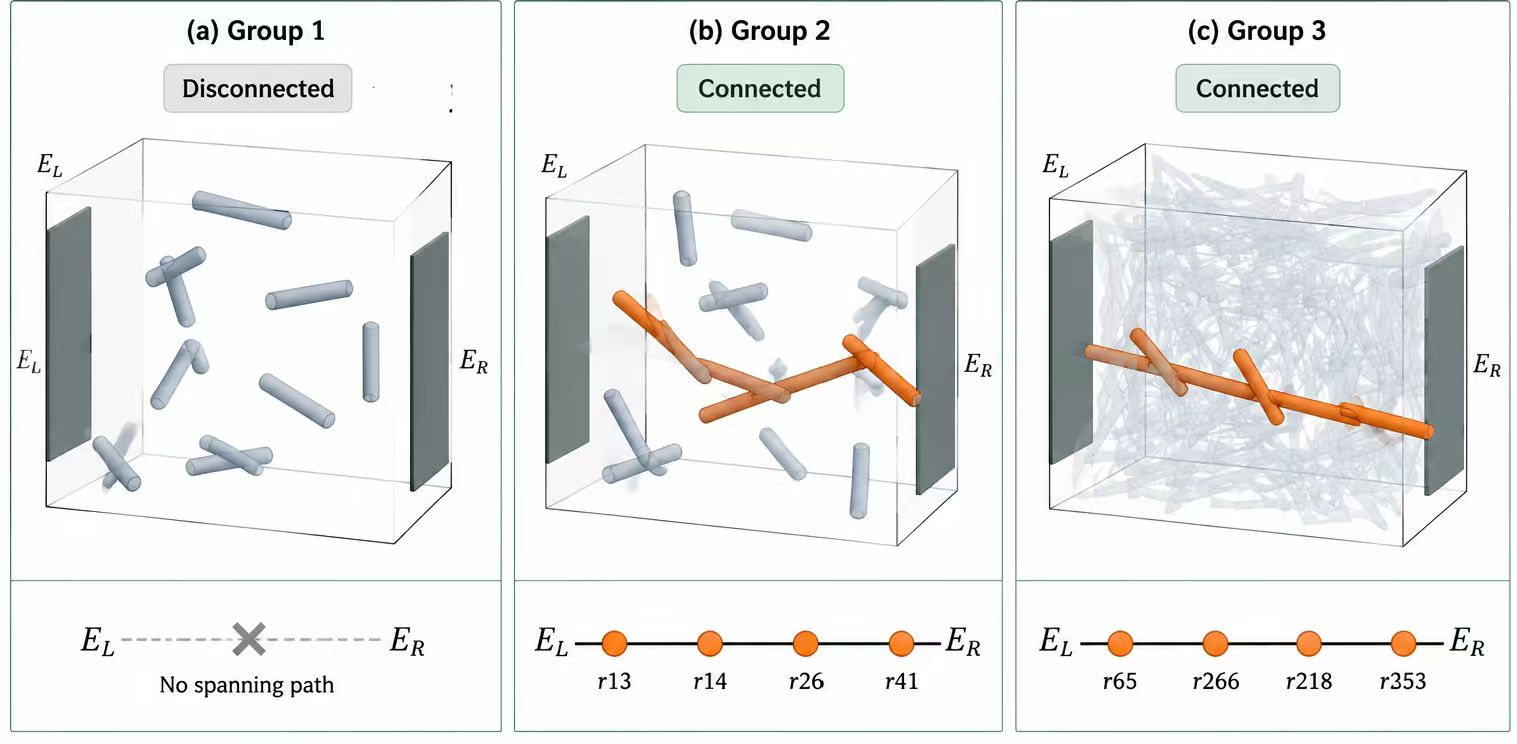
\includegraphics[width=0.98\textwidth]{figures/q1_contact_witness.jpg}
  \caption{附件三组微构体的电极贯通结构与接触图见证。灰色片段为背景片段，橙色片段为电极间见证片段，深灰面为电极，圆点连线表示接触图中的拓扑边；组 1 无跨接路径，组 2 与组 3 沿图示片段导通。两片段间的几何距离满足 $d_{ij}\le\delta=1.8\,\mathrm{nm}$ 时，在接触图中加入边 $(i,j)\in E$。图中结构与接触关系为示意，未按比例绘制。}
  \label{fig:q1-groups}
\end{figure}

\begin{figure}[H]
  \centering
  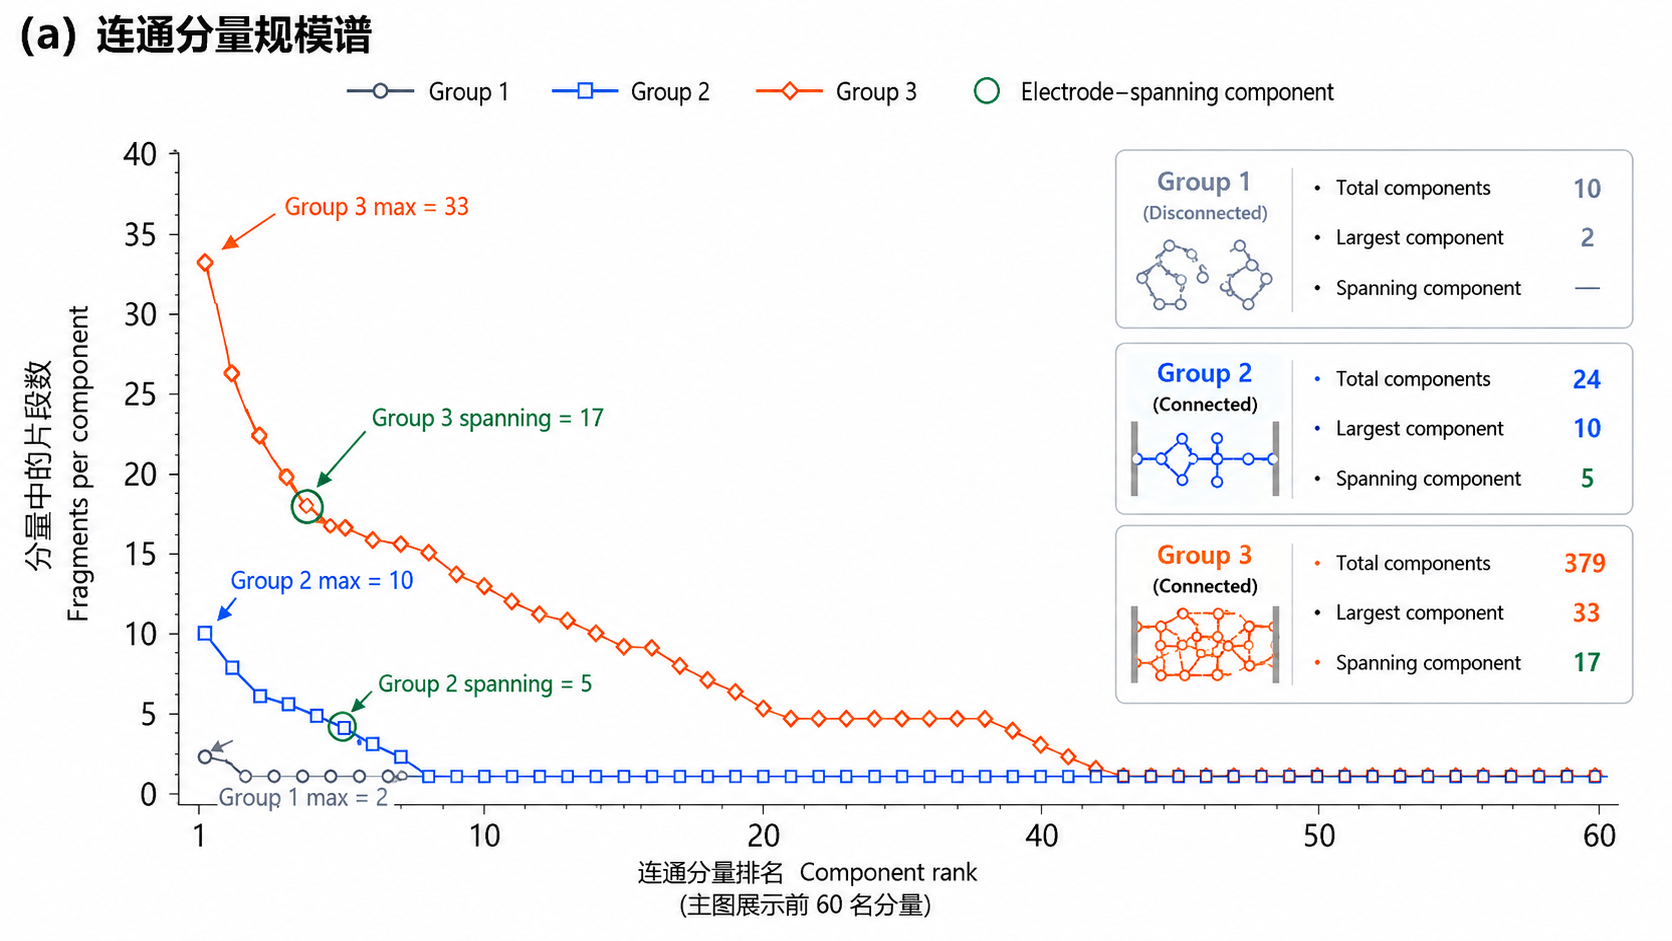
\includegraphics[width=0.98\textwidth]{figures/q1_component_spectrum.png}
  \caption{\textbf{三组接触网络的连通分量规模谱。}灰、蓝、橙曲线分别给出组 1--3 按规模降序排列的前 60 个连通分量，右侧汇总分量总数、最大分量及贯通分量规模；绿色圆圈标出连接左右电极的贯通分量。组 1 不导通，组 2 和组 3 的贯通分量分别含 5 个和 17 个片段。}
  \label{fig:q1-contact-network}
\end{figure}

\FloatBarrier

\subsection{5.2 问题二：四个 A 填充量的导通概率}\label{ux95eeux9898ux4e8cux56dbux4e2a-a-ux586bux5145ux91cfux7684ux5bfcux901aux6982ux7387}

\subsubsection{5.2.1 粒子数换算与试验设置}\label{ux7c92ux5b50ux6570ux6362ux7b97ux4e0eux8bd5ux9a8cux8bbeux7f6e}

A 的单粒子名义体积和微构体体积为

\[
V_A=\pi r_A^2\ell_A=4.5\times10^6\pi\ \mathrm{nm^3},\qquad
V_\Omega=10^{12}\ \mathrm{nm^3}.
\]

对目标名义体积分数 \(\phi\)，粒子数取

\[
N_A=\operatorname{round}\!\left(\frac{\phi V_\Omega}{V_A}\right),\qquad
\phi_{\mathrm{actual}}(N_A)=100\%\times\frac{N_AV_A}{V_\Omega}.
\]

按题意四舍五入后，\(0.50\%,0.60\%,0.70\%,1.00\%\) 分别对应 \(N_A=354,424,495,707\)。 整数化后的实际体积分数略有偏差，正文同时报告目标值与离散实际值，并以整数粒子数计算概率。

正式模拟采用 \(n=20000\) 次独立试验，根种子为 \(20260801\)；每次试验生成至 \(N_{\max}=720\) 的有序 A 粒子序列。四个查询点共享同一组首次导通时刻 \(T_s\)，不同试验的中心和方向相互独立。达到 720 根仍不导通的 90 次试验记为右删失值 721；对本问任一 \(N\leq707\)，事件 \(T_s\leq N\) 的计数不受右删失影响。

\subsubsection{5.2.2 概率估计结果}\label{ux6982ux7387ux4f30ux8ba1ux7ed3ux679c}

由 \(k_N=\#\{s:T_s\leq N\}\) 直接计数，并按第 4.4 节计算双侧 \(95\%\) Wilson 区间，得到：

\begingroup
\small
\setlength{\tabcolsep}{3pt}
\begin{table}[H]
\centering
\caption{四个题给 A 填充量的导通概率估计}
\begin{tabular}{@{}
  >{\centering\arraybackslash}p{(\linewidth - 10\tabcolsep) * \real{0.19}}
  >{\centering\arraybackslash}p{(\linewidth - 10\tabcolsep) * \real{0.09}}
  >{\centering\arraybackslash}p{(\linewidth - 10\tabcolsep) * \real{0.17}}
  >{\centering\arraybackslash}p{(\linewidth - 10\tabcolsep) * \real{0.12}}
  >{\centering\arraybackslash}p{(\linewidth - 10\tabcolsep) * \real{0.12}}
  >{\centering\arraybackslash}p{(\linewidth - 10\tabcolsep) * \real{0.31}}@{}}
\toprule
题给体积分数 & 粒子数 & 实际体积分数 & 导通次数 & 概率估计 & \(95\%\) Wilson 区间 \\
\midrule
\(0.50\%\) & 354 & \(0.500456\%\) & 1579 & \(7.895\%\) & \([7.529\%,8.277\%]\) \\
\(0.60\%\) & 424 & \(0.599416\%\) & 4410 & \(22.050\%\) & \([21.481\%,22.630\%]\) \\
\(0.70\%\) & 495 & \(0.699790\%\) & 9439 & \(47.195\%\) & \([46.504\%,47.887\%]\) \\
\(1.00\%\) & 707 & \(0.999498\%\) & 19856 & \(99.280\%\) & \([99.153\%,99.388\%]\) \\
\bottomrule
\end{tabular}
\end{table}
\endgroup

四个点的经验概率依次为 \(7.895\%,22.050\%,47.195\%,99.280\%\)。从 \(0.50\%\) 到 \(0.70\%\)，导通概率快速上升；到 \(1.00\%\) 时已有 \(19856/20000\) 个微构体导通，形成清晰的 S 形有限尺寸贯通过渡。各点均由蒙特卡洛成功次数直接计数；共同前缀使每次试验内四个导通指标保持单调，从而稳定呈现概率跃迁顺序。

概率曲线和问题三的临界整数联合置信判定见图 \ref{fig:q2-q3-curve}。

\begin{figure}[htbp]
  \centering
  
\includegraphics[width=\textwidth]{figures/q2_q3_probability.png}
  \caption{全 A 介质导通概率与临界区联合认证。(a) 问题二全范围导通概率曲线及四个题给填充量；(b) 问题三临界整数的单侧联合置信判定。}
  \label{fig:q2-q3-curve}
\end{figure}

\subsection{5.3 问题三：全 A 的最低填充量}\label{ux95eeux9898ux4e09ux5168-a-ux7684ux6700ux4f4eux586bux5145ux91cf}

\subsubsection{5.3.1 从经验临界点到概率约束}\label{ux4eceux7ecfux9a8cux4e34ux754cux70b9ux5230ux6982ux7387ux7ea6ux675f}

对一条预先生成的无限 A 介质序列，前 \(N\) 根构成填充量为 \(N\) 的设计。增加介质只会向接触图 加入节点和边，不会删除已有通路，因而真实导通概率 \(p_A(N)\) 关于 \(N\) 单调不减。问题三的 理想整数目标为

\[
N_A^\star=\min\{N\in\mathbb Z_{\ge0}:p_A(N)\ge0.90\}.
\]

样本比例在 \(90\%\) 附近时，本文以联合校正单侧精确限作为正式门槛。\(N_A=613,\ldots,616\) 的全 A 设计与相邻 A/B 配比共同构成 41 个设计的完整确认集，并统一使用 \(100000\) 次试验。每次试验生成一张最大静态图，各设计共享同一随机构型；不同试验彼此独立。这一结构同时保留设计间的配对比较和试验间的伯努利独立性。

\subsubsection{5.3.2 精确单侧界与联合置信控制}\label{ux7cbeux786eux5355ux4fa7ux754cux4e0eux8054ux5408ux7f6eux4fe1ux63a7ux5236}

对固定的 \(N\)，令 \(K_N=\sum_{s=1}^{n}Y_s(N)\)。在模型给定的随机机制下， \(K_N\sim\operatorname{Bin}(n,p_A(N))\)。Clopper--Pearson 方法通过反解二项分布尾概率得到 置信限{[}6{]}；若 \(B^{-1}(q;a,b)\) 表示 Beta 分布的 \(q\) 分位数，则

\[
p_L^{\mathrm{CP}}=B^{-1}(\alpha_i;K_N,n-K_N+1),\qquad
p_U^{\mathrm{CP}}=B^{-1}(1-\alpha_i;K_N+1,n-K_N).
\]

该方法由二项分布尾概率直接给出有限样本覆盖保证。对 41 个设计各使用一个单侧下限，取

\[
\alpha_i=\frac{0.05}{41}=0.001219512\ldots.
\]

记第 \(j\) 个置信陈述失效的事件为 \(E_j\)。由 Bonferroni 不等式{[}7{]}，

\[
\Pr\!\left(\bigcup_{j=1}^{41}E_j\right)
\le \sum_{j=1}^{41}\Pr(E_j)\le41\alpha_i=0.05.
\]

所以全部 41 个下限同时成立的概率至少为 \(95\%\)。Bonferroni 联合界允许设计间相关，适用于共享最大静态图的配对结构。若 \(p_L^{\mathrm{CP}}\geq0.90\)，则记为达标；否则记为未达标。

\subsubsection{5.3.3 确认结果与题定精度}\label{ux786eux8ba4ux7ed3ux679cux4e0eux9898ux5b9aux7cbeux5ea6}

四个全 A 设计的结果见表 \ref{tab:q3-confirmation}。所有成功数均由同一组 \(100000\) 次试验的最大静态图一次汇总得到，表中精确限采用 41 项 Bonferroni 校正。

\begin{table}[htbp]
  \centering
  \small
  \caption{统一样本中的全 A 临界设计}
  \label{tab:q3-confirmation}
  \begin{tabular}{cccccc}
    \toprule
    $N_A$ & 成功数 & 经验概率 & CP 单侧下限 & CP 单侧上限 & 联合判定 \\
    \midrule
    613 & 89965 & $89.965\%$ & $89.6739\%$ & $90.2509\%$ & 未达标 \\
    614 & 90189 & $90.189\%$ & $89.9008\%$ & $90.4720\%$ & 未达标 \\
    615 & 90403 & $90.403\%$ & $90.1176\%$ & $90.6832\%$ & 可行 \\
    616 & 90601 & $90.601\%$ & $90.3182\%$ & $90.8786\%$ & 可行 \\
    \bottomrule
  \end{tabular}
\end{table}

613、614 根的联合校正下限低于 \(90\%\)，615、616 根达到正式门槛。由于共同前缀保证成功数及 其 Clopper--Pearson 下限随粒子数单调不减，615 根是正式联合置信判据下的最小可行整数，即

\[
N_A^\star=615,
\]

由 \(V_A=0.0045\pi\ \mathrm{\mu m^3}\) 与 \(V_\Omega=1000\ \mathrm{\mu m^3}\)，其名义体积分数为

\[
100\%\frac{615V_A}{V_\Omega}=0.8694357669\%\approx\mathbf{0.87\%}.
\]

故按题目百分号后两位的口径，问题三的最优方案为 \textbf{\(0.87\%\)、615 根 A}。其经验导通 概率为 \(90.403\%\)、41 项校正单侧下限为 \(90.1176\%\)、成本为 \(9.1290755523\) 元。

\subsection{5.4 问题四：A/B 混合填充的正整数成本优化}\label{ux95eeux9898ux56dbab-ux6df7ux5408ux586bux5145ux7684ux6b63ux6574ux6570ux6210ux672cux4f18ux5316}

\subsubsection{5.4.1 正整数可行域与精确成本权重}\label{ux6b63ux6574ux6570ux53efux884cux57dfux4e0eux7cbeux786eux6210ux672cux6743ux91cd}

题目要求同时填充介质 A 和介质 B，因此本问的决策域为 \(N_A,N_B\in\mathbb Z_{\ge1}\)。两类单粒子的名义体积和成本分别为

\[
V_A=0.0045\pi\ \mathrm{\mu m^3},\quad
V_B=\frac{0.032\pi}{3}\ \mathrm{\mu m^3},\qquad
c_A=\frac{189\pi}{40000}\ \text{元},\quad
c_B=\frac{\pi}{1875}\ \text{元}.
\]

于是概率约束整数规划写为

\[
\min_{N_A,N_B\in\mathbb Z_{\ge1}} C=c_AN_A+c_BN_B,
\qquad \text{s.t.}\quad p(N_A,N_B)\ge0.90.
\]

利用 \(c_A/c_B=567/64\)，将成本化为整数权重

\[
W(N_A,N_B)=567N_A+64N_B,\qquad C=\frac{\pi}{120000}W.
\]

这样可以无浮点误差地比较任意两个设计。B 的单位名义体积价格较低，而 A 的长径比达到 \(l_A/(2r_A)=83.33\)，具有更强的长程搭桥能力；成本优化同时权衡局部填充价格与长程拓扑连通能力。

对 B 的越界部分，球心为 \(c\)、胞索引为 \(k\in\{-1,0,1\}^3\) 时，映回基础域的球片为

\[
K_k=\bigl(\operatorname{Ball}(c,r_B)\cap(\Omega+kL)\bigr)-kL
=\operatorname{Ball}(c-kL,r_B)\cap\Omega.
\]

每个非空球片独立成为凸体节点。完整球对使用闭式距离，涉及球片的接触使用支持映射与 GJK 判定，从而与 A 的截断片段独立规则保持一致。

\subsubsection{5.4.2 二维 minimax 路径前沿}\label{ux4e8cux7ef4-minimax-ux8defux5f84ux524dux6cbf}

对第 \(s\) 次试验，只构建一次最大前缀对应的静态接触图 \(G_s^{\max}\)。记激活阈值 \(\tau(v)=(\tau_A(v),\tau_B(v))\)：由第 \(i\) 个 A 介质产生的片段赋值为 \((i,0)\)，由第 \(j\) 个 B 介质产生的片段赋值为 \((0,j)\)，左右电极均取 \((0,0)\)。对于任意一条连接两电极的路径 \(P\)，定义其二维 minimax 标签为

\[
\ell(P)=\left(
\max_{v\in P}\tau_A(v),
\max_{v\in P}\tau_B(v)
\right).
\]

标签 \(\ell(P)=(a,b)\) 表示该路径能够出现所需的最小 A、B 前缀规模。若两个标签满足

\[
a_1\leq a_2,\qquad b_1\leq b_2,
\]

则称 \((a_1,b_1)\) 支配 \((a_2,b_2)\)。被支配标签不会对应更早激活的贯通路径，因此可以在传播过程中删除。

从左电极开始传播标签，并在每个节点仅保留 Pareto 非支配集合。右电极处最终得到的前沿记为 \(\mathcal F_s\)，则设计 \((N_A,N_B)\) 在第 \(s\) 次试验中的导通状态满足

\[
Y_s(N_A,N_B)=1
\Longleftrightarrow
\exists(a,b)\in\mathcal F_s:\quad
a\leq N_A,\ b\leq N_B.
\]

因此，一张最大静态图及其二维前沿即可批量查询多个整数配比，无须为每个设计重新计算几何接触关系。该表示还直接保证 \(Y_s(N_A,N_B)\) 分别关于 \(N_A\) 和 \(N_B\) 单调不减。

\subsubsection{5.4.3 低成本候选域与联合确认}\label{ux4f4eux6210ux672cux5bb6ux65cfux51bbux7ed3ux4e0eux72ecux7acbux786eux8ba4}

根据问题三得到的全 A 临界区域，将混合介质候选限制在 \(N_A=613,614,615\)，并以 \(C(615,4)\) 为成本上界。定义正整数混合候选集

\[
\mathcal D_+=\left\{
(N_A,N_B):
N_A\in\{613,614,615\},\quad
N_B\in\mathbb Z_{\geq1},\quad
C(N_A,N_B)\leq C(615,4)
\right\}.
\]

由精确整数成本权重 \(W=567N_A+64N_B\) 可得

\[
\begin{aligned}
N_A=613 &: \quad N_B=1,\ldots,21,\\
N_A=614 &: \quad N_B=1,\ldots,12,\\
N_A=615 &: \quad N_B=1,\ldots,4.
\end{aligned}
\]

因此 \(\mathcal D_+\) 共包含 \(21+12+4=37\) 个混合配比。另取

\[
\mathcal R_A=\{(613,0),(614,0),(615,0),(616,0)\}
\]

作为全 A 参照，最终确认集合为

\[
\mathcal D=\mathcal D_+\cup\mathcal R_A,
\qquad |\mathcal D|=41.
\]

集合 \(\mathcal R_A\) 用于连接问题三与问题四的结果，不属于同时填充 A、B 的正整数混合可行域。

每次试验构建最大前缀 \((616,21)\) 对应的静态图，再利用二维非支配前沿同时查询确认集合 \(\mathcal D\) 中的 41 个设计。各设计共享同一个随机构型，因而可以进行配对比较；不同试验之间保持独立。正式确认采用 \(100000\) 个固定随机构型。

对每个设计计算 Bonferroni 校正的单侧 Clopper--Pearson 下限，单项显著性水平为

\[
\alpha_i=\frac{0.05}{41}.
\]

若未舍入的置信下限满足

\[
p_L^{\mathrm{CP}}\geq0.90,
\]

则将该设计判为已确认可行。十个连续的 \(10000\) 样本分块仅用于检查结果波动，正式判定始终采用完整的 \(100000\) 次试验。

\subsubsection{5.4.4 候选域内的最低成本方案}\label{ux56faux5b9aux5bb6ux65cfux5185ux7684ux6210ux672cux63a8ux8350}

在确认集合 \(\mathcal D\) 中，共有 19 个设计的 Bonferroni 校正单侧 Clopper--Pearson 下限达到 \(90\%\)。在正整数混合候选集 \(\mathcal D_+\) 内，成本最低的已确认可行设计为

\[
(N_A,N_B)=(614,6).
\]

其成功次数、经验导通概率、联合校正下限和成本分别为

\[
k_{614,6}=90302,
\qquad
\widehat p=\frac{90302}{100000}=90.302\%,
\]

\[
p_L^{\mathrm{CP}}=90.0153\%,
\qquad
C=9.1242846235\ \text{元}.
\]

与其相邻的较低成本设计 \((614,5)\) 的经验导通概率为 \(90.282\%\)，但校正后的单侧下限为

\[
89.9950\%<90\%,
\]

未通过正式可行判据。增加一个 B 介质后，\((614,6)\) 的置信下限越过 \(90\%\) 门槛，因此它构成当前候选域内最低成本的已确认可行混合方案。

问题三得到的全 A 参照 \((615,0)\) 具有

\[
\widehat p=90.403\%,
\qquad
p_L^{\mathrm{CP}}=90.1176\%,
\qquad
C=9.1290755523\ \text{元}.
\]

与该全 A 方案相比，\((614,6)\) 以少一根 A 和六个 B 达到相同的概率约束，并将已确认可行成本由 \(9.1291\) 元降至 \(9.1243\) 元。

\begin{table}[htbp]
  \centering
  \small
  \caption{低成本候选域的门槛设计与全 A 参照}
  \label{tab:q4-confirmation}
  \setlength{\tabcolsep}{3pt}
  \renewcommand{\arraystretch}{1.02}
  \renewcommand{\tabularxcolumn}[1]{>{\centering\arraybackslash}m{#1}}
  \begin{tabularx}{\textwidth}{cXccccc}
    \toprule
    配比 & 证据角色 & 成功数 & 经验概率 & CP 单侧下限 & 描述性 CP 上限 & 成本（元） \\
    \midrule
    $(614,5)$ & 较低成本相邻设计 & $90282/100000$ & $90.282\%$ & $89.9950\%$ & $90.5638\%$ & $9.1226091074$ \\
    $(614,6)$ & 候选域内最低成本可行设计 & $90302/100000$ & $90.302\%$ & $90.0153\%$ & $90.5835\%$ & $9.1242846235$ \\
    $(615,0)$ & 问题三全 A 参照 & $90403/100000$ & $90.403\%$ & $90.1176\%$ & $90.6832\%$ & $9.1290755523$ \\
    \bottomrule
  \end{tabularx}
\end{table}

\begin{figure}[htbp]
  \centering
  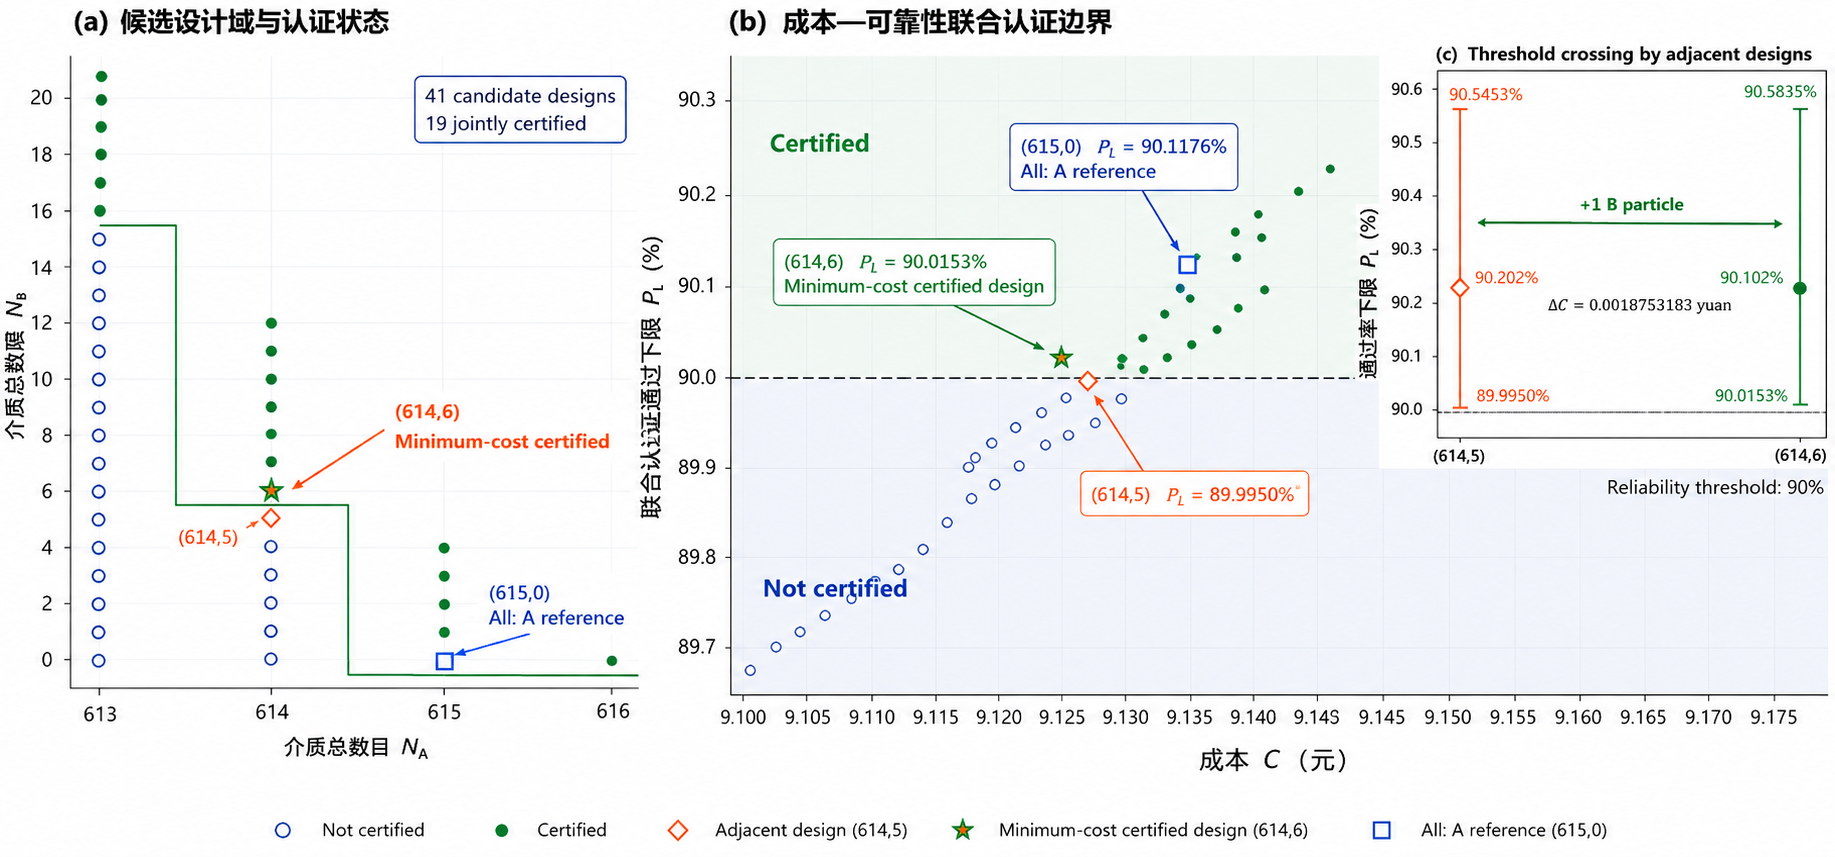
\includegraphics[width=\textwidth]{figures/q4_cost_frontier_user_selected.png}
  \caption{\textbf{预先确定的低成本设计集合及其联合确认结果。}(a) 37 个正整数混合候选和 4 个全 A 参照在 $(N_A,N_B)$ 平面中的判定状态；(b) 设计成本与 Bonferroni 校正单侧 Clopper--Pearson 下限，虚线为 $90\%$ 可行门槛；(c) 相邻设计 $(614,5)$ 与 $(614,6)$ 的经验概率及单侧置信限。星号表示混合候选域内成本最低的已确认可行设计。}
  \label{fig:q4-cost-frontier}
\end{figure}

为核查统计可行性所对应的实际空间通路，从 \((614,6)\) 的正式试验中选取首个导通构型，分别重建其全局轴测结构和局部贯通路径。图中橙色片段构成恢复得到的电极间见证链，蓝色点表示介质 B；三维图件用于核验空间构型与接触关系，不参与概率估计。

\begin{figure}[htbp]
  \centering
  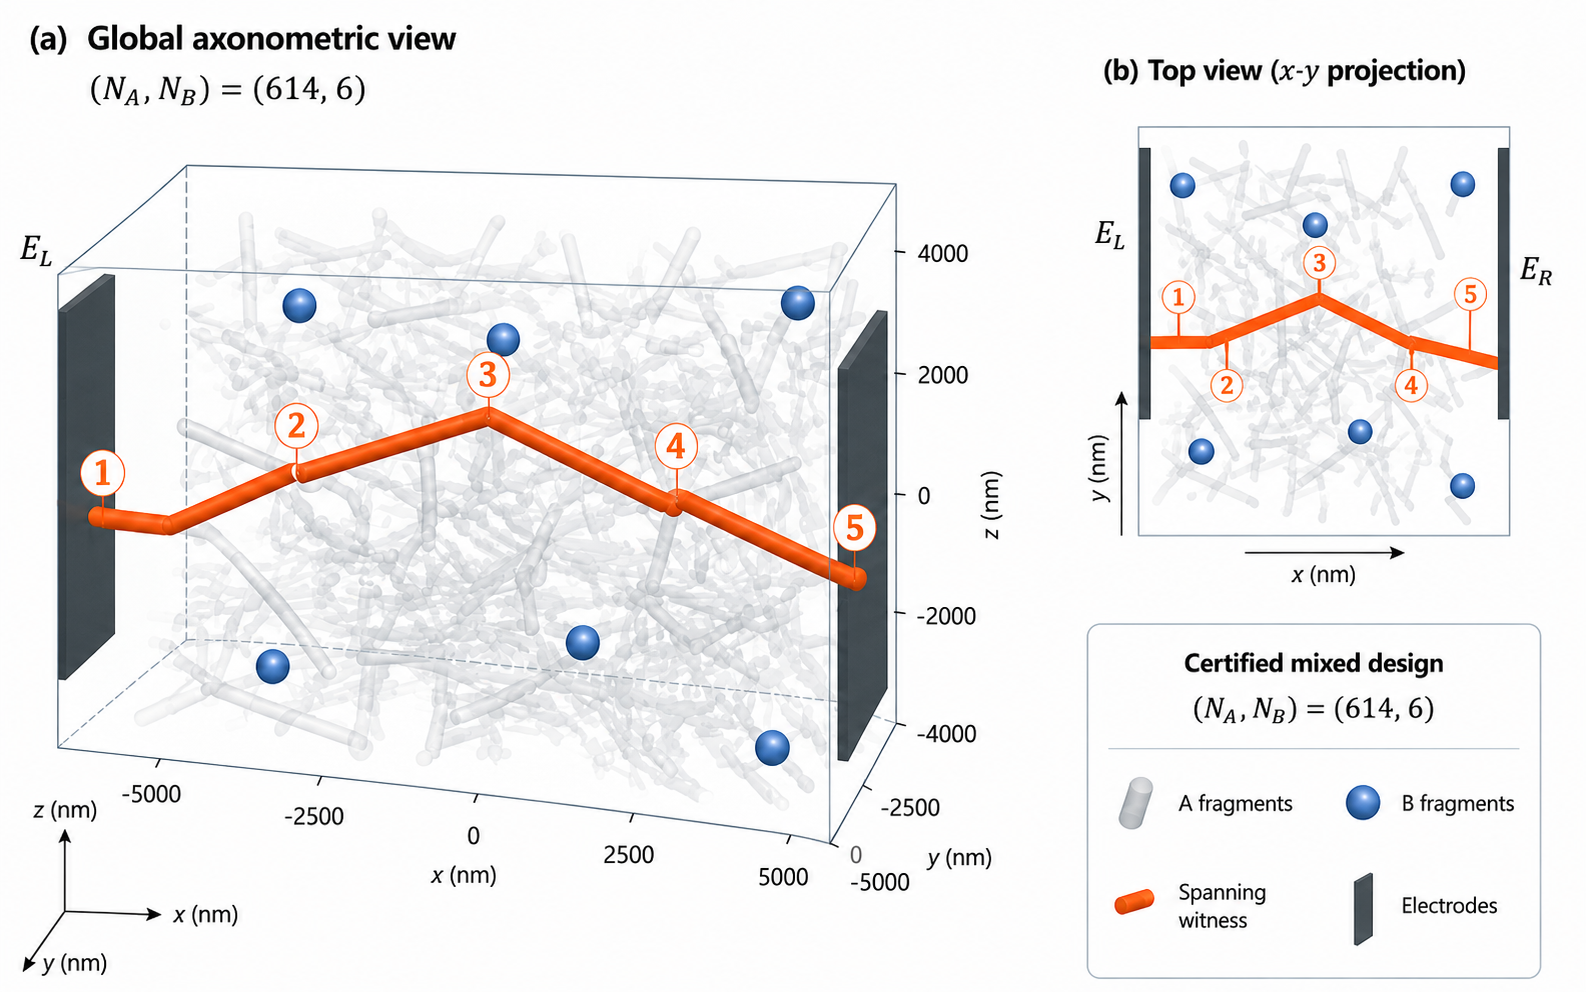
\includegraphics[width=0.90\textwidth]{figures/q4_optimal_global_user_selected.png}
  \caption{候选域内最低成本的已确认可行配比 $(614,6)$ 的全局构型与俯视投影。(a) 全局轴测重建；(b) 同一构型在 $x$--$y$ 平面上的俯视投影。浅灰色圆柱为 A 片段，蓝色球体为 B 片段，橙色圆柱为程序恢复的实际贯通见证；数字 $1$--$5$ 标示见证片段从左电极到右电极的顺序。}
  \label{fig:q4-global-3d}
\end{figure}

\begin{figure}[htbp]
  \centering
  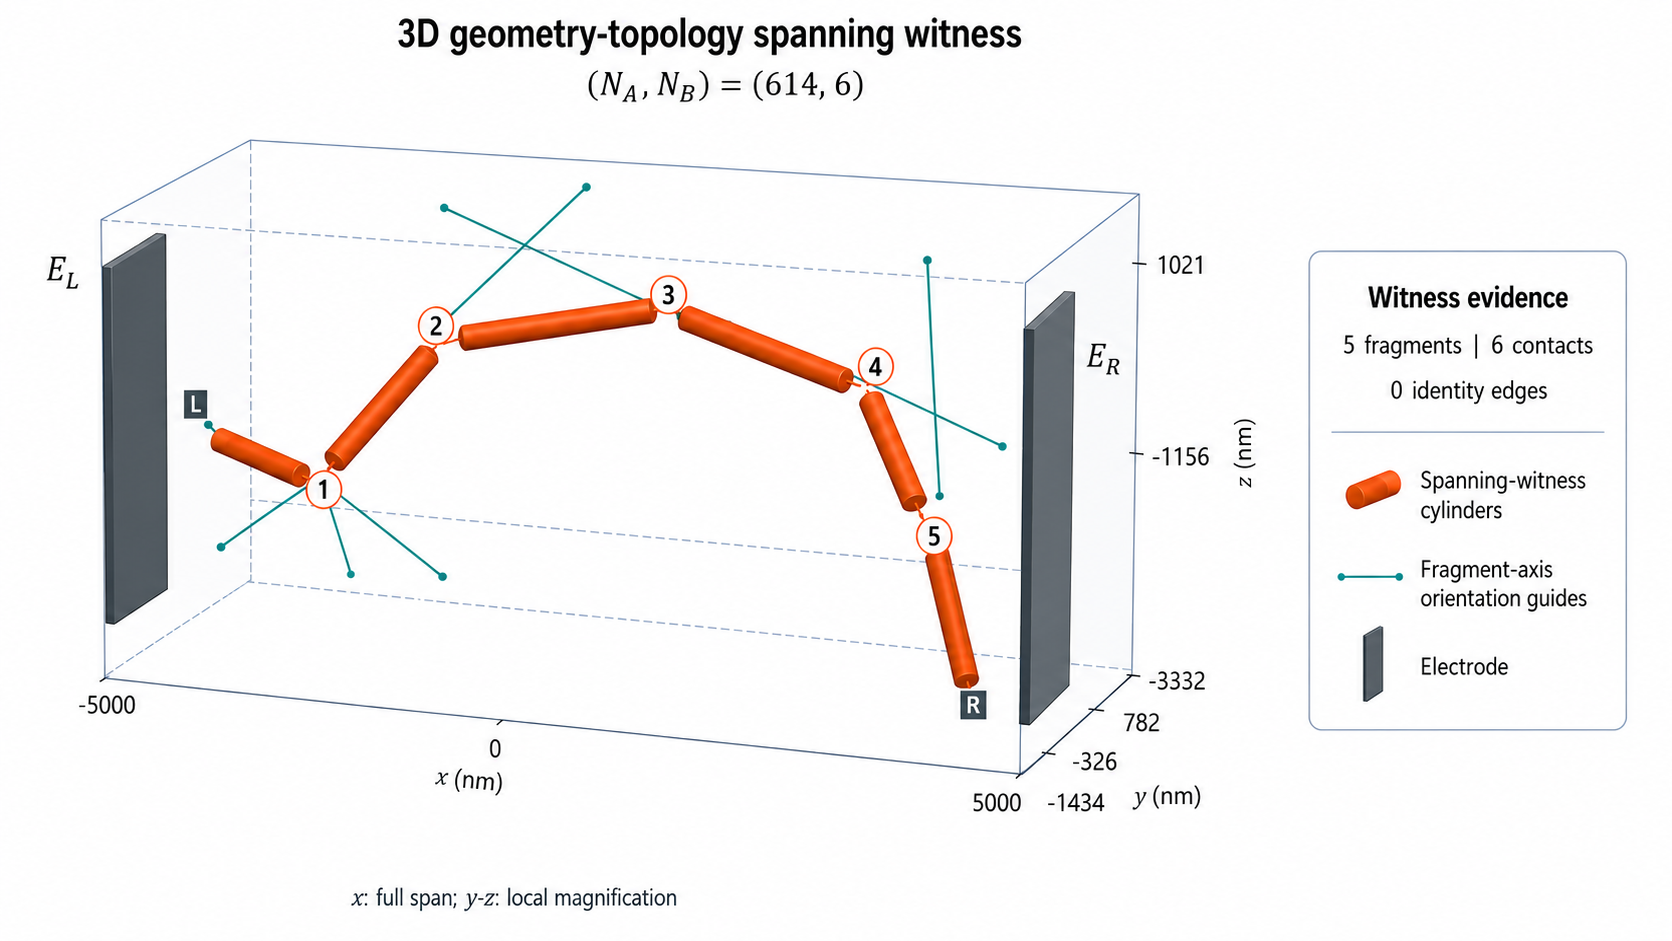
\includegraphics[width=0.98\textwidth]{figures/q4_optimal_witness_user_selected.png}
  \caption{配比 $(614,6)$ 的局部三维几何--拓扑贯通见证。橙色圆柱链按 $L\to1\to2\to3\to4\to5\to R$ 展示有序贯通关系，青绿色细线标示五个见证片段的轴向；该见证包含 5 个片段节点与 6 条已核验接触关系，同源内部边为 0。}
  \label{fig:q4-witness-3d}
\end{figure}
\FloatBarrier

\section{六、模型检验与结果讨论}\label{ux516dux6a21ux578bux68c0ux9a8cux4e0eux7ed3ux679cux8ba8ux8bba}

\subsection{6.1 几何核与图算法}\label{ux51e0ux4f55ux6838ux4e0eux56feux7b97ux6cd5ux68c0ux9a8c}

\textbf{几何距离核检验。}针对平底圆柱，距离核测试覆盖了平行侧面、垂直相交、端面对端、实体贯穿、电极接触，以及 \(1.8\pm\varepsilon\,\mathrm{nm}\) 接触阈值邻域等典型构型。对每一对候选实体，GJK 算法同步维护真实距离的下界 \(L\) 与上界 \(U\)：当 \(U\le\delta\) 时判定为接触，当 \(L>\delta\) 时判定为分离；若 \(L\le\delta<U\)，则继续收紧数值容差，直至得到确定的分类结果。球片支持映射的检验覆盖球内、单面截断、棱截断和角截断等情形；对于完整球--球和圆柱--球组合，则采用闭式距离公式进行计算。

\textbf{图算法一致性检验。}Union--Find 与 BFS 对左右电极是否贯通的判定逐例一致，表明基于接触边合并的并查集算法与基于路径搜索的连通性检验得到了相同结果。进一步将二维 minimax 非支配标签前沿算法与完整整数网格上的全量搜索（exhaustive search）进行对照，所有设计点的导通状态均保持一致。对于确认集合 \(\mathcal D\) 中的 \(41\) 个设计，又依次核验了路径激活阈值、蒙特卡洛成功计数和联合置信判定，未发现任何结果不一致的情况。

\subsection{6.2 随机模拟与统计判定}\label{ux968fux673aux6a21ux62dfux4e0eux7edfux8ba1ux68c0ux9a8c}

\textbf{各向同性随机生成检验。}设随机生成的方向向量为

\[
\mathbf u=(u_x,u_y,u_z),
\]

理论上应满足

\[
\mathbb E[u_x]=\mathbb E[u_y]=\mathbb E[u_z]=0,
\]

以及

\[
\mathbb E[u_x^2]=\mathbb E[u_y^2]=\mathbb E[u_z^2]=\frac13.
\]

数值检验表明，三个方向分量的一阶矩和二阶矩经验值均与上述理论结果相符，说明方向采样满足各向同性要求。

\textbf{样本量与置信区间解释。}当 \(p\approx0.9\)、\(n=100000\) 时，未经多重比较校正的比例标准误约为

\[
\sqrt{\frac{p(1-p)}{n}}\approx 0.000949,
\]

即约 \(0.0949\) 个百分点。经 Bonferroni 校正后，设计 \((614,5)\) 与 \((614,6)\) 的单侧 Clopper--Pearson 下限分别为 \(89.9950\%\) 和 \(90.0153\%\)，恰好分居 \(90\%\) 判定门槛两侧。正式分类均依据未舍入的精确下限进行，表中小数仅用于结果展示。由于每个设计的样本量预先固定为 \(100000\)，并对确认集合中的 \(41\) 项判定实施联合校正，因此所得区间可按照固定样本量条件下的联合覆盖概率进行解释{[}8{]}。

\textbf{共同随机数结构。}在问题二的同一次随机试验中，不同设计共享相同的 A 粒子前缀；问题三和问题四则基于同一张最大静态图开展计算，使全 A 设计与混合设计能够在相同随机构型下形成配对比较。不同蒙特卡洛试验之间相互独立，而同一试验内的不同设计共享底层构型，从而提高统计效率，并增强不同设计结果之间的可比性。

\subsection{6.3 跨问题一致性}\label{ux8de8ux95eeux9898ux4e00ux81f4ux6027ux4e0eux8bc1ux636eux5c42ux7ea7}

问题三与问题四沿用了相同的 D 边界语义、A 类粒子几何模型和 \(1.8\ \mathrm{nm}\) 接触阈值，并统一纳入确认集合 \(\mathcal D\) 的联合统计判定。在全 A 参照集 \(\mathcal R_A\) 中，\(N_A=613,614,615,616\) 时的导通成功次数分别为 \(89965,90189,90403,90601\)。以 \(N_A=615\) 为例，其经验导通率为 \(90.403\%\)，Bonferroni 校正后的单侧置信下限为 \(90.1176\%\)。因此，\(N_A=615\) 是全 A 整数设计中首个通过 \(90\%\) 门槛的方案，对应的最低填充量为 \(0.87\%\)。

确认集合 \(\mathcal D\) 中共有 \(19\) 个设计达到联合置信下限门槛。在正整数混合候选域 \(\mathcal D_+\) 内，成本最低的已确认可行方案为 \((614,6)\)。该方案在 \(100000\) 次模拟中成功导通 \(90302\) 次，经验导通概率为 \(90.302\%\)，校正后的单侧置信下限为 \(90.0153\%\)，对应成本为 \(9.1242846235\) 元。与其相邻的设计 \((614,5)\) 的校正下限为 \(89.9950\%\)，尚未达到 \(90\%\) 门槛，由此形成了清晰的临界对照。

\subsection{6.4 模型适用条件与拓展}\label{ux9002ux7528ux8303ux56f4ux4e0eux7ed3ux679cux8fb9ux754c}

本文模型适用于题设几何尺寸与随机生成机制：接触阈值取 \(\delta=1.8\,\mathrm{nm}\)，介质中心独立均匀分布，A 的轴向服从球面各向同性分布，粒子允许重叠，填充量按名义体积计算，并采用截断片段相互独立的 D 边界规则。核心输出为左右贯通事件及其概率；接入接触电阻、隧穿衰减和路径并联参数后，同一图模型可继续计算等效电导率。

B 越界球片由球与胞盒的真实凸交表示，A 越界片段则按圆柱中心线与盒面的交点切分为有限平底圆柱。两类实体均通过支持映射参与凸体距离计算，因此若进一步采用解析半空间裁剪或 CAD 布尔交提高 A 边界几何的描述精度，宽相筛选、GJK 窄相判定与图连通搜索的主体流程仍可保持不变。对于边界处理方式或接触阈值的调整，可在相应几何口径下重新构建接触图，并据此更新导通概率、临界填充量及成本优化结果。

\section{七、模型评价与结论}\label{ux4e03ux6a21ux578bux8bc4ux4ef7ux4e0eux7ed3ux8bba}

\begingroup
\small
\subsection{7.1 模型优点}\label{ux6a21ux578bux4f18ux70b9}

\begin{enumerate}
\def\labelenumi{\arabic{enumi}.}
\tightlist
\item
  \textbf{几何与路径一致。}模型保留有限平底圆柱、球和球片的凸几何，宽相作候选排除，窄相用距离上下界分类，贯通见证直接由接触图恢复。
\item
  \textbf{一套接触图贯穿四问。}确定性附件、随机概率、一维临界填充和二维混合成本共享同一 几何语义与接触判据。共同前缀和二维路径阈值复用最大图，把重复计算转化为增量查询，同时从 算法结构上保证粒子数单调性。
\item
  \textbf{统计结论与优化结论统一。}对确认集合 \(\mathcal D\) 中的 \(41\) 个设计使用相同的固定样本，Clopper--Pearson 精确界处理有限样本，Bonferroni 控制全部单侧陈述。问题三据此确定最小全 A 填充量，问题四给出正整数混合候选域 \(\mathcal D_+\) 内最低成本的已确认可行设计。
\item
  \textbf{结果可复现。}固定种子和试验序号唯一确定随机输入，串行与并行计算得到相同结果；关键概率、置信限、成本和三维见证均可由计算程序重复得到。
\end{enumerate}

\subsection{7.2 模型拓展}\label{ux5c40ux9650ux4e0eux6539ux8fdbux65b9ux5411}

现有统一接触图框架可直接扩展到解析半空间裁剪或 CAD 布尔交，以重建有限半径圆柱的完整边界 片；共同随机数随后量化几何升级对临界粒子数和问题四低成本临界带的影响。实验图像与工艺数据 可进一步标定取向、团聚和排斥过程，形成面向真实制备条件的参数化随机模型。

几何间距、接触面积和界面电阻可转化为边电导，再由 Kirchhoff 网络求解等效电导率；对 \((614,5)\) 与 \((614,6)\) 所在窄临界带，增加固定样本并细化整数网格即可进一步提高门槛分辨率。

\subsection{7.3 结论}\label{ux7ed3ux8bba}

问题一的三个附件微构体依次为\textbf{不导通、导通、导通}，两个导通组均给出了从左电极到右电极 的逐边见证。问题二在 20000 次固定试验下，\(0.50\%\)、\(0.60\%\)、\(0.70\%\)、\(1.00\%\) 四个 名义体积分数对应的导通概率依次为 \textbf{\(7.895\%\)、\(22.050\%\)、\(47.195\%\)、\(99.280\%\)}。

问题三的全 A 设计得到：\(615\) 根的经验导通率为 \textbf{\(90.403\%\)}，经 \(41\) 项联合校正后的单侧下限为 \textbf{\(90.1176\%\)}，是首个达到门槛的整数设计；最小填充量为 \textbf{\(0.87\%\)}。

问题四在确认集合 \(\mathcal D\) 中得到 19 个达标设计。正整数混合候选域 \(\mathcal D_+\) 内成本最低的已确认可行配比为 \textbf{\((614,6)\)}，经验导通概率 \textbf{90.302\%}、校正单侧下限 \textbf{90.0153\%}、成本 \textbf{9.1243 元}。

\TemplateMatterHeading{AI 工具使用声明}

本参赛队在竞赛过程中使用了 OpenAI Codex{[}9{]}，主要用于资料检索、程序实现检查、代码调试、 图表生成和语言整理，详细使用情况见附录 A。核心模型、数学推导、参数口径、数值结果和结论 均由参赛队复核。

\endgroup
\TemplateMatterHeading{参考文献}
\begingroup
\zihao{-5}

{[}1{]} GILBERT E G, JOHNSON D W, KEERTHI S S. A fast procedure for computing the distance between complex objects in three-dimensional space{[}J{]}. IEEE Journal on Robotics and Automation, 1988, 4(2): 193-203. DOI:10.1109/56.2083.

{[}2{]} BALBERG I, ANDERSON C H, ALEXANDER S, et al.~Excluded volume and its relation to the onset of percolation{[}J{]}. Physical Review B, 1984, 30(7): 3933-3943. DOI:10.1103/PhysRevB.30.3933.

{[}3{]} LORENZ C D, ZIFF R M. Precise determination of the critical percolation threshold for the three-dimensional ``Swiss cheese'' model using a growth algorithm{[}J{]}. The Journal of Chemical Physics, 2001, 114(8): 3659-3661. DOI:10.1063/1.1338506.

{[}4{]} NEWMAN M E J, ZIFF R M. Fast Monte Carlo algorithm for site or bond percolation{[}J{]}. Physical Review E, 2001, 64(1): 016706. DOI:10.1103/PhysRevE.64.016706.

{[}5{]} WILSON E B. Probable inference, the law of succession, and statistical inference{[}J{]}. Journal of the American Statistical Association, 1927, 22(158): 209-212. DOI:10.1080/01621459.1927.10502953.

{[}6{]} CLOPPER C J, PEARSON E S. The use of confidence or fiducial limits illustrated in the case of the binomial{[}J{]}. Biometrika, 1934, 26(4): 404-413. DOI:10.1093/biomet/26.4.404.

{[}7{]} DUNN O J. Multiple comparisons among means{[}J{]}. Journal of the American Statistical Association, 1961, 56(293): 52-64. DOI:10.1080/01621459.1961.10482090.

{[}8{]} HOWARD S R, RAMDAS A, MCAULIFFE J, et al.~Time-uniform, nonparametric, nonasymptotic confidence sequences{[}J{]}. The Annals of Statistics, 2021, 49(2): 1055-1080. DOI:10.1214/20-AOS1991.

{[}9{]} OPENAI. Codex{[}EB/OL{]}. 2026.

\endgroup
\clearpage
\TemplateMatterHeading{附录}

\subsection{附录 A：AI 工具使用详情}\label{ux9644ux5f55-aai-ux5de5ux5177ux4f7fux7528ux8be6ux60c5}

使用工具为 OpenAI Codex，开发机构为 OpenAI，使用日期为 2026-08-07 至 2026-08-08。工具主要用于程序检查、图表生成和语言整理，模型、推导、数值与结论均由参赛队复核。

{\def\LTcaptype{none} % do not increment counter
\small
\setlength{\tabcolsep}{4pt}
\begin{longtable}[]{@{}
  >{\raggedright\arraybackslash}p{(\linewidth - 6\tabcolsep) * \real{0.1800}}
  >{\raggedright\arraybackslash}p{(\linewidth - 6\tabcolsep) * \real{0.2800}}
  >{\raggedright\arraybackslash}p{(\linewidth - 6\tabcolsep) * \real{0.2600}}
  >{\raggedright\arraybackslash}p{(\linewidth - 6\tabcolsep) * \real{0.2800}}@{}}
\toprule\noalign{}
\begin{minipage}[b]{\linewidth}\raggedright
使用环节
\end{minipage} & \begin{minipage}[b]{\linewidth}\raggedright
关键 Prompt 摘要
\end{minipage} & \begin{minipage}[b]{\linewidth}\raggedright
回复摘要
\end{minipage} & \begin{minipage}[b]{\linewidth}\raggedright
采纳内容与人工核验
\end{minipage} \\
\midrule\noalign{}
\endhead
\bottomrule\noalign{}
\endlastfoot
规则与模板 & 阅读赛题、格式规范和官方 Word 模板，列出硬性提交要求 & 给出页边距、首页、页码、页数、匿名与文件命名检查项 & 参赛队逐页对照官方模板完成版式核验 \\
建模与推导 & 按题意建立有限实体接触、图连通和概率约束模型 & 给出凸体距离、共同随机前缀、整数成本和联合置信路线 & 参赛队重推公式，并以特殊构型、量纲和单调性检查 \\
程序与仿真 & 实现可复现的几何核、Monte Carlo 和概率约束求解 & 生成或修改 Python 程序、单元测试和运行命令 & 固定随机种子，运行全部测试并抽查原始样本与汇总结果 \\
图表与三维建模 & 依据计算结果生成统计图和 FreeCAD 三维模型 & 辅助生成绘图、CAD 构建和渲染脚本 & 参赛队逐项核对图中数据、三维对象数量和空间接触关系 \\
论文整理 & 将正式证据组织为摘要、正文、参考文献和附录 & 辅助压缩文字、统一符号并构建 LaTeX & 参赛队核对全部数值与结论；按官方 Word 模板核验版式并逐页检查 LaTeX PDF 后定稿 \\
\end{longtable}
}

论文中的概率、置信限、成本和三维场景均由可执行程序生成；参赛队复核文献、程序、图件与最终结论。

\subsection{附录 B：软件环境与复现说明}\label{ux9644ux5f55-bux8f6fux4ef6ux73afux5883ux4e0eux590dux73b0ux547dux4ee4}

计算环境为 Windows 11、Python 3.13、NumPy、SciPy、Numba、Matplotlib 和 pytest；三维模型使用 FreeCAD 1.1.1；论文由 XeLaTeX 编译，并按官方 Word 模板逐页核验。根随机种子固定为 \texttt{20260801}，问题二使用 \(20000\) 次独立试验，问题三、四对 41 个整数设计统一使用 \(100000\) 次试验。

复现顺序为：先运行几何与图算法测试，再完成问题一的确定性接触判定；随后生成问题二的共同前缀样本、问题三的临界整数结果和问题四的二维成本结果；最后重建统计图、三维见证并编译论文。完整程序随支撑材料提交。

\noindent\textbf{源码生成说明：} 本附录由冻结提交源码清单自动生成，共列入 24 个程序；代码内容与正式提交源码逐字节一致。当前仅因组别与参赛编号未填写而标记为 INTERNAL-QA。\par
\vspace{0.4em}
\Needspace{6\baselineskip}
\subsection{附录 C.1 项目级复现入口}
\noindent{}原项目相对路径：\texttt{run\_pipeline.py}\par
\vspace{0.25em}
{\fontsize{6.4pt}{7.2pt}\selectfont
\VerbatimInput[breaklines=true,breakanywhere=true,numbers=left,numbersep=5pt,frame=single,framesep=2mm,rulecolor=\color{black!35}]{source_appendix/001.py}
}
\Needspace{6\baselineskip}
\subsection{附录 C.2 附件分段重建与审计程序}
\noindent{}原项目相对路径：\texttt{02\_数据与参数/src/reconstruct\_segments.py}\par
\vspace{0.25em}
{\fontsize{6.4pt}{7.2pt}\selectfont
\VerbatimInput[breaklines=true,breakanywhere=true,numbers=left,numbersep=5pt,frame=single,framesep=2mm,rulecolor=\color{black!35}]{source_appendix/002.py}
}
\Needspace{6\baselineskip}
\subsection{附录 C.3 问题一有限圆柱接触与导通判定程序}
\noindent{}原项目相对路径：\texttt{问题/问题1/src/solve.py}\par
\vspace{0.25em}
{\fontsize{6.4pt}{7.2pt}\selectfont
\VerbatimInput[breaklines=true,breakanywhere=true,numbers=left,numbersep=5pt,frame=single,framesep=2mm,rulecolor=\color{black!35}]{source_appendix/003.py}
}
\Needspace{6\baselineskip}
\subsection{附录 C.4 问题二固定样本蒙特卡洛程序}
\noindent{}原项目相对路径：\texttt{问题/问题2/src/solve.py}\par
\vspace{0.25em}
{\fontsize{6.4pt}{7.2pt}\selectfont
\VerbatimInput[breaklines=true,breakanywhere=true,numbers=left,numbersep=5pt,frame=single,framesep=2mm,rulecolor=\color{black!35}]{source_appendix/004.py}
}
\Needspace{6\baselineskip}
\subsection{附录 C.5 问题三两阶段概率确认程序}
\noindent{}原项目相对路径：\texttt{问题/问题3/src/solve.py}\par
\vspace{0.25em}
{\fontsize{6.4pt}{7.2pt}\selectfont
\VerbatimInput[breaklines=true,breakanywhere=true,numbers=left,numbersep=5pt,frame=single,framesep=2mm,rulecolor=\color{black!35}]{source_appendix/005.py}
}
\Needspace{6\baselineskip}
\subsection{附录 C.6 问题四混合介质成本优化程序}
\noindent{}原项目相对路径：\texttt{问题/问题4/src/solve.py}\par
\vspace{0.25em}
{\fontsize{6.4pt}{7.2pt}\selectfont
\VerbatimInput[breaklines=true,breakanywhere=true,numbers=left,numbersep=5pt,frame=single,framesep=2mm,rulecolor=\color{black!35}]{source_appendix/006.py}
}
\Needspace{6\baselineskip}
\subsection{附录 C.7 有限平底圆柱几何核}
\noindent{}原项目相对路径：\texttt{公共代码/geometry\_kernel.py}\par
\vspace{0.25em}
{\fontsize{6.4pt}{7.2pt}\selectfont
\VerbatimInput[breaklines=true,breakanywhere=true,numbers=left,numbersep=5pt,frame=single,framesep=2mm,rulecolor=\color{black!35}]{source_appendix/007.py}
}
\Needspace{6\baselineskip}
\subsection{附录 C.8 几何窄相加速核}
\noindent{}原项目相对路径：\texttt{公共代码/fast\_geometry.py}\par
\vspace{0.25em}
{\fontsize{6.4pt}{7.2pt}\selectfont
\VerbatimInput[breaklines=true,breakanywhere=true,numbers=left,numbersep=5pt,frame=single,framesep=2mm,rulecolor=\color{black!35}]{source_appendix/008.py}
}
\Needspace{6\baselineskip}
\subsection{附录 C.9 单介质随机微构体仿真核}
\noindent{}原项目相对路径：\texttt{公共代码/microstructure\_sim.py}\par
\vspace{0.25em}
{\fontsize{6.4pt}{7.2pt}\selectfont
\VerbatimInput[breaklines=true,breakanywhere=true,numbers=left,numbersep=5pt,frame=single,framesep=2mm,rulecolor=\color{black!35}]{source_appendix/009.py}
}
\Needspace{6\baselineskip}
\subsection{附录 C.10 混合介质随机微构体仿真核}
\noindent{}原项目相对路径：\texttt{公共代码/mixed\_microstructure\_sim.py}\par
\vspace{0.25em}
{\fontsize{6.4pt}{7.2pt}\selectfont
\VerbatimInput[breaklines=true,breakanywhere=true,numbers=left,numbersep=5pt,frame=single,framesep=2mm,rulecolor=\color{black!35}]{source_appendix/010.py}
}
\Needspace{6\baselineskip}
\subsection{附录 C.11 二维资源连通与 Pareto 前沿算法}
\noindent{}原项目相对路径：\texttt{公共代码/pareto\_connectivity.py}\par
\vspace{0.25em}
{\fontsize{6.4pt}{7.2pt}\selectfont
\VerbatimInput[breaklines=true,breakanywhere=true,numbers=left,numbersep=5pt,frame=single,framesep=2mm,rulecolor=\color{black!35}]{source_appendix/011.py}
}
\Needspace{6\baselineskip}
\subsection{附录 C.12 结果注册与 LaTeX 导出程序}
\noindent{}原项目相对路径：\texttt{公共代码/result\_registry.py}\par
\vspace{0.25em}
{\fontsize{6.4pt}{7.2pt}\selectfont
\VerbatimInput[breaklines=true,breakanywhere=true,numbers=left,numbersep=5pt,frame=single,framesep=2mm,rulecolor=\color{black!35}]{source_appendix/012.py}
}
\Needspace{6\baselineskip}
\subsection{附录 C.13 科学绘图样式模块}
\noindent{}原项目相对路径：\texttt{公共代码/plot\_style.py}\par
\vspace{0.25em}
{\fontsize{6.4pt}{7.2pt}\selectfont
\VerbatimInput[breaklines=true,breakanywhere=true,numbers=left,numbersep=5pt,frame=single,framesep=2mm,rulecolor=\color{black!35}]{source_appendix/013.py}
}
\Needspace{6\baselineskip}
\subsection{附录 C.14 问题一三维场景数据生成程序}
\noindent{}原项目相对路径：\texttt{论文/figures/src/build\_q1\_scenes.py}\par
\vspace{0.25em}
{\fontsize{6.4pt}{7.2pt}\selectfont
\VerbatimInput[breaklines=true,breakanywhere=true,numbers=left,numbersep=5pt,frame=single,framesep=2mm,rulecolor=\color{black!35}]{source_appendix/014.py}
}
\Needspace{6\baselineskip}
\subsection{附录 C.15 FreeCAD 参数化实体建模程序}
\noindent{}原项目相对路径：\texttt{论文/figures/src/build\_freecad\_scene.py}\par
\vspace{0.25em}
{\fontsize{6.4pt}{7.2pt}\selectfont
\VerbatimInput[breaklines=true,breakanywhere=true,numbers=left,numbersep=5pt,frame=single,framesep=2mm,rulecolor=\color{black!35}]{source_appendix/015.py}
}
\Needspace{6\baselineskip}
\subsection{附录 C.16 FreeCAD 通用视图渲染程序}
\noindent{}原项目相对路径：\texttt{论文/figures/src/render\_freecad\_scene.py}\par
\vspace{0.25em}
{\fontsize{6.4pt}{7.2pt}\selectfont
\VerbatimInput[breaklines=true,breakanywhere=true,numbers=left,numbersep=5pt,frame=single,framesep=2mm,rulecolor=\color{black!35}]{source_appendix/016.py}
}
\Needspace{6\baselineskip}
\subsection{附录 C.17 问题二与问题三概率图生成程序}
\noindent{}原项目相对路径：\texttt{论文/figures/src/build\_q2\_q3\_figure.py}\par
\vspace{0.25em}
{\fontsize{6.4pt}{7.2pt}\selectfont
\VerbatimInput[breaklines=true,breakanywhere=true,numbers=left,numbersep=5pt,frame=single,framesep=2mm,rulecolor=\color{black!35}]{source_appendix/017.py}
}
\Needspace{6\baselineskip}
\subsection{附录 C.18 问题四成本前沿图生成程序}
\noindent{}原项目相对路径：\texttt{论文/figures/src/build\_q4\_frontier.py}\par
\vspace{0.25em}
{\fontsize{6.4pt}{7.2pt}\selectfont
\VerbatimInput[breaklines=true,breakanywhere=true,numbers=left,numbersep=5pt,frame=single,framesep=2mm,rulecolor=\color{black!35}]{source_appendix/018.py}
}
\Needspace{6\baselineskip}
\subsection{附录 C.19 问题四真实随机试验三维建模程序}
\noindent{}原项目相对路径：\texttt{论文/figures/src/build\_q4\_mixed\_scene.py}\par
\vspace{0.25em}
{\fontsize{6.4pt}{7.2pt}\selectfont
\VerbatimInput[breaklines=true,breakanywhere=true,numbers=left,numbersep=5pt,frame=single,framesep=2mm,rulecolor=\color{black!35}]{source_appendix/019.py}
}
\Needspace{6\baselineskip}
\subsection{附录 C.20 问题四三维场景渲染与审计程序}
\noindent{}原项目相对路径：\texttt{论文/figures/src/render\_q4\_mixed\_scene.py}\par
\vspace{0.25em}
{\fontsize{6.4pt}{7.2pt}\selectfont
\VerbatimInput[breaklines=true,breakanywhere=true,numbers=left,numbersep=5pt,frame=single,framesep=2mm,rulecolor=\color{black!35}]{source_appendix/020.py}
}
\Needspace{6\baselineskip}
\subsection{附录 C.21 问题四导通见证与有序接触图生成程序}
\noindent{}原项目相对路径：\texttt{论文/figures/src/build\_q4\_witness\_figure.py}\par
\vspace{0.25em}
{\fontsize{6.4pt}{7.2pt}\selectfont
\VerbatimInput[breaklines=true,breakanywhere=true,numbers=left,numbersep=5pt,frame=single,framesep=2mm,rulecolor=\color{black!35}]{source_appendix/021.py}
}
\Needspace{6\baselineskip}
\subsection{附录 C.22 问题四正式三维资产串行生成与总审计程序}
\noindent{}原项目相对路径：\texttt{论文/figures/src/build\_q4\_final\_assets.py}\par
\vspace{0.25em}
{\fontsize{6.4pt}{7.2pt}\selectfont
\VerbatimInput[breaklines=true,breakanywhere=true,numbers=left,numbersep=5pt,frame=single,framesep=2mm,rulecolor=\color{black!35}]{source_appendix/022.py}
}
\Needspace{6\baselineskip}
\subsection{附录 C.23 问题四正式确认完整整数域独立审计程序}
\noindent{}原项目相对路径：\texttt{问题/问题4/src/audit\_confirmation.py}\par
\vspace{0.25em}
{\fontsize{6.4pt}{7.2pt}\selectfont
\VerbatimInput[breaklines=true,breakanywhere=true,numbers=left,numbersep=5pt,frame=single,framesep=2mm,rulecolor=\color{black!35}]{source_appendix/023.py}
}
\Needspace{6\baselineskip}
\subsection{附录 C.24 统一建模流程与验证诊断图生成程序}
\noindent{}原项目相对路径：\texttt{论文/figures/src/build\_explanatory\_figures.py}\par
\vspace{0.25em}
{\fontsize{6.4pt}{7.2pt}\selectfont
\VerbatimInput[breaklines=true,breakanywhere=true,numbers=left,numbersep=5pt,frame=single,framesep=2mm,rulecolor=\color{black!35}]{source_appendix/024.py}
}



\end{document}
